% THESIS.TEX -- main file for the dissertation, built on the offline
% uonthesis document class (University of Nottingham).
\documentclass[11pt]{uonthesis}

% Explicitly force A4 -- the class does not set a paper size itself,
% so without this the compiler's default is used, which on some
% servers (e.g. Overleaf) is US Letter rather than A4.
\setlength{\paperwidth}{210mm}
\setlength{\paperheight}{297mm}
\special{papersize=210mm,297mm} % dvips/older engines
\ifx\pdfpagewidth\undefined\else
  \pdfpagewidth=\paperwidth
  \pdfpageheight=\paperheight
\fi

\usepackage[titletoc]{appendix}
\usepackage{graphicx}

% ---- Additional packages needed for the dissertation content ----
\usepackage{amsmath}
\usepackage{amssymb}
\usepackage{amsthm}
\usepackage{booktabs}
\usepackage{array}
\usepackage{tabularx}
\usepackage{caption}
\usepackage{subcaption}
\usepackage{xcolor}
\usepackage{algorithm}
\usepackage{algpseudocode}
\usepackage{enumitem}
\usepackage{float}
\usepackage[authoryear,round]{natbib}
\providecommand{\newblock}{\hskip .11em plus .33em minus .07em}
\usepackage{hyperref}
\usepackage[capitalise]{cleveref}

\bibliographystyle{plainnat} % author-year style, matches \citep/\citet/\citeauthor below

\hypersetup{
    colorlinks=true,
    linkcolor=blue!50!black,
    citecolor=green!50!black,
    urlcolor=blue!50!black,
    breaklinks=true,
    pdftitle={Adaptive Geodesic Conformal Prediction for Uncertainty-Quantified Spherical Harmonic Reconstruction of Climate Fields},
    pdfauthor={Sze Ying Choong}
}
\urlstyle{same} % render URLs in the body text font instead of monospace

\newcommand{\R}{\mathbb{R}}
\newcommand{\dgeo}{d_{\mathrm{geo}}}
% ---- End additions ----

% Patch: avoid a trailing comma on the title page when \prevdegrees{} is empty
% Patch: add \studentid and \supervisor fields (not provided by the base class)
\makeatletter
\def\studentid#1{\gdef\@studentid{#1}}
\def\supervisor#1{\gdef\@supervisor{#1}}
\def\@studentid{}
\def\@supervisor{}
\def\maketitle{
{\ssp
\begin{alwayssingle}
    \let\footnotesize\small
    \let\footnoterule\relax
    \thispagestyle{empty}
    \setcounter{page}{1}
    \null\vfil
    \vskip 40pt
  \begin{center}
    
\includegraphics[width=0.55\textwidth]{images/nottingham-logo}
    \vskip 2.5em
    {\huge {\@title} \par}
    \vskip 3em
    {\Large
     \lineskip .75em
     by {\@author}\ifx\@prevdegrees\@empty\else, {\@prevdegrees}\fi \par}
    \ifx\@studentid\@empty\else
      \vskip .5em
      {\large Student ID: {\@studentid} \par}
    \fi
    \vskip 3em
           {\Large
             Submitted to {\@university} \par\smallskip {\@date} \par\smallskip
             in partial fulfilment of the conditions for the
             award of the degree of \par\smallskip{\@degree} \par
             \vfill}
    \ifx\@supervisor\@empty\else
      {\large Supervised by {\@supervisor} \par}
      \vskip 1.5em
    \fi
            {\normalsize I declare that this dissertation is all my own work,
             except as indicated in the text
           }
  \end{center}
  \vfil\null
\end{alwayssingle}
\setcounter{footnote}{0}
}}

% Patch: the class's \abstract macro opens with \null\vfil, which pushes the
% "Abstract" heading down using stretchable glue that consumes the whole page,
% leaving no room for the actual abstract text (it was overflowing onto the
% next page). Remove that leading \vfil so the heading sits at the top and
% the text flows immediately below it, matching how \acknowledgements behaves.
\def\abstract{
 \def\ps@BCplain{\let\@mkboth\@gobbletwo
      \def\@oddhead{}\def\@oddfoot{\rm\hfil\thepage
      \hfil}\def\@evenhead{}\let\@evenfoot\@oddfoot}
\begin{alwayssingle}
\thispagestyle{BCplain}
\begin{center}
{\large \bfseries \abstractname}
\end{center}}
\def\endabstract{\par\vfil\null\end{alwayssingle}}
\makeatother

\renewcommand{\appendixtocname}{List of appendices}

\title{Adaptive Geodesic Conformal Prediction for Uncertainty-Quantified Spherical Harmonic Reconstruction of Climate Fields}
\author{Sze Ying Choong}
\prevdegrees{} % no prior degree listed
\university{The University of Nottingham}
\degree{Master in Data Science}
\date{10 September 2026}
\studentid{20798235}
\supervisor{Dr.\ Luis Espath}

%%%%%%%%%%%%%%%%%%%%%%%%%%%%%%%%%%%%%%%%%%%%%%%%%%%%%%%%%%%%%%%%%%%%%%%%%%%%%%%%%%%%
\begin{document}

\begin{frontmatter}
\maketitle
\tableofcontents

\begin{abstract}
This dissertation adds an uncertainty quantification layer to a reconstructed continuous field on a sphere from sparse, scattered observations. This is relevant to areas such as climate science, geophysics, and computer graphics, where uncertainty is important for real-world applications.

From earlier research, the physics-informed spherical harmonic model developed by Thomas (2025) uses a regularised spherical harmonic expansion with a Sobolev-type seminorm penalty to produce accurate point reconstructions of global temperature from city-level data. However, it provides no information about the reliability of these predictions. 

Therefore, adaptive geodesic conformal prediction was applied as an additional layer to the existing spherical harmonic pipeline. Since temperature is scalar rather than manifold-valued, spherical geometry enters through the input locations rather than the output. By using great-circle distances on the sphere, a cross-validated nearest-neighbour estimator was used to estimate the local reconstruction difficulty, $\hat{\sigma}(x)$. The conformal scores are then normalised by $\hat{\sigma}(x)$ before calibration so that the resulting prediction interval width varies according to local data density and local reconstruction difficulty.

This project used Berkeley Earth city-temperature observations, with $n=3,510$ observations from July 2003. The standard conformal prediction method achieved an overall coverage close to the nominal 90\%; however, significant differences were observed across difficulty levels. The lowest-difficulty tertile achieved 100\% coverage, whereas the highest-difficulty tertile achieved only 76.7\%. In contrast, the adaptive method produced more balanced coverage across three tertiles, between 91\% and 95\%. The adaptive method produced a narrower mean prediction interval of 4.59°C, compared with 4.65°C for the standard method. Overall, the adaptive method provides more reliable local uncertainty estimates while maintaining a similar mean interval width. 

A robustness experiment across spherical harmonic degrees from L=8 to L=30 showed that the adaptive method continued to perform well across different model complexities. The highest-uncertainty locations were mainly concentrated in the high-altitude Andes, where local observation coverage was relatively sparse. This may indicate that the estimated uncertainty captures aspects of spatial data sparsity and provides useful insight into where reconstruction predictions may be less reliable.

\noindent \textbf{Keywords:} spherical harmonics; conformal prediction; uncertainty quantification; climate field reconstruction; geodesic distance; adaptive calibration; spatial statistics; Sobolev regularisation

\end{abstract}

\begin{acknowledgements}

First of all, I am very thankful to my supervisor, Luis Espath. He guided me throughout this project and supported my ideas and findings. He gave me precise feedback and helpful suggestions that helped me stay on track with the topic. In particular, I found the mathematical and methodological aspects difficult to understand at first. Through our meetings and discussions, however, I was able to understand these aspects better, and the project progressed more smoothly.

Besides this, I would also like to thank Thomas Will (2025), who developed the spherical harmonic reconstruction framework. His work provided the starting point and foundation for my dissertation. I used the existing reconstruction model as the base predictor and then focused on adding uncertainty quantification and conformal prediction on top of it. This allowed me to focus on the new uncertainty component rather than rebuilding the reconstruction model from scratch. He was also kind enough to explain his previous code to me and answer my questions about his dissertation. His comments on my implementation was very helpful in shaping and improving my dissertation.

Last but not least, I would like to thank my family and friends for their support and encouragement throughout my MSc. They supported me and cheered me up during difficult times. Their encouragement meant a lot to me and helped me get through the challenging periods while completing this dissertation.


\end{acknowledgements}

\listoffigures
\listoftables

\end{frontmatter}

%%%%%%%%%%%%%%%%%%%%%%%%%%%%%%%%%%%%%%%%%%%%%%%%%%%%%%%%%%%%%%%%%%%%%%%%%%%%%%%%%%%%
\chapter{Introduction}
\label{ch:intro}

\section{Motivation}

Many scientific quantities are defined on the surface of a sphere, $S^2$, such as surface temperature, geomagnetic fields, atmospheric pressure, gravitational potential, and wind direction. In reality, we do not observe the field continuously. Instead, observations are finite, scattered, and often spatially irregular. Weather stations, satellite measurements, and survey sites are some examples of observation sources. The main problem here is to reconstruct a continuous field from sparse observations while also determining how trustworthy it is at each location.

Spherical harmonics are a natural basis for reconstructing fields on a sphere due to their properties of orthogonality, completeness for square-integrable functions on the sphere, and their relationship with the spherical Laplace-Beltrami operator. These properties allow the model to control the smoothness or roughness of the reconstructed field with Sobolev-type regularisation. The predecessor dissertation by Thomas (2025) developed regularised spherical harmonic reconstruction for scalar fields and vector fields using vector spherical harmonics. The previous work, which was applied to real global temperature and wind data, showed good reconstruction accuracy. It also showed that the choice of spherical harmonic degree $L$ affects the balance between model complexity and the available data \citep{thomas2025}. Regularisation in this case helps prevent overfitting, while different regularisation seminorms can effectively control model smoothness. The existing model performs well for point prediction, but uncertainty is still missing.

For example, users need to know whether the prediction is likely to be within $0.5^\circ\mathrm{C}$ or whether the actual value could differ by $10^\circ\mathrm{C}$. This is especially important in difficult areas with sparse observations, such as oceans and polar regions, as well as regions with strong or local physical variability. In this dissertation, the high-altitude Andes become an important finding, suggesting that uncertainty is important for identifying where the reconstruction is reliable and where it is difficult.

This concern is not only related to our temperature dataset. A reconstructed field may be used for downstream purposes such as deciding where more monitoring is needed, feeding climate information into another model, supporting agricultural or environmental analysis, and communicating predictions to non-specialists. The quality of the reconstructed field may therefore affect decision-making in real-life applications. Therefore, users need to know how much they should trust a prediction at a particular location. A single global RMSE only provides information on how well the model performs on average; it does not tell us about the model's performance at a specific location. These two questions can have very different answers when, as is generally true of spatial data, prediction error is heteroscedastic across the domain. In other words, prediction difficulty can vary across the domain, leading to heteroscedastic prediction errors. Therefore, global accuracy metrics alone are insufficient for understanding local reliability.

This motivates spatially adaptive uncertainty quantification. Conformal prediction is selected because it is model-agnostic and does not require a specific probability distribution for the model errors. It can be easily applied to an existing predictor, while its coverage guarantee is based on exchangeability rather than assuming that the base model is correctly specified.

So, why not Gaussian processes or Kriging? They are also established approach to spatial uncertainty quantification that can provide a predictive distribution at each location. However, they require assumptions about the underlying stochastic process, covariance structure, and choice of kernel. If the covariance or kernel is misspecified, the uncertainty estimates may become poorly calibrated. Standard GP methods can also become computationally expensive as the number of observations increases. Standard GP inference typically scales approximately as $O(n^3)$. Instead, conformal prediction provides a different approach that does not require the base predictor to be probabilistic and can work well with the existing spherical harmonic model. It does not require redesigning the reconstruction model and provides a formal marginal coverage guarantee under exchangeability. Therefore, conformal prediction is preferred for this dissertation.

\section{Contributions}

This dissertation extends the spherical harmonic reconstruction framework of \citet{thomas2025} with a spatially adaptive uncertainty quantification layer. It is built by adapting the adaptive geodesic conformal prediction framework of \citet{amirishahbazi2026}, which uses a manifold-valued response in regression problems (e.g.\ a direction on $S^2$). However, the climate reconstruction problem is scalar, making this adaptation different. This adaptation is novel because the geodesic structure of the sphere is used to define a spatially local difficulty estimator $\hat\sigma(x)$ over the input domain. The estimator is obtained using cross-validated $k$-nearest-neighbour regression on residuals based on great-circle distance, and the conformal scores for the scalar output are normalised by this estimator. The contributions of this dissertation are separated into five parts:

\begin{enumerate}
    \item \textbf{Methodological adaptation} - Move geodesic information from the manifold response to the spherical input locations for scalar temperature (\cref{sec:adaptation}).
    \item \textbf{New uncertainty layer} - Add local $\hat{\sigma}(x)$ estimation and adaptive conformal calibration to the existing spherical harmonic model.
    \item \textbf{Empirical validation} - Show better coverage across regions with different levels of difficulty while maintaining similar interval widths.
    \item \textbf{Robustness} - Test different $L$ values using two hyperparameter-selection criteria for $\lambda$.
    \item \textbf{Geographic interpretation} - Show that high uncertainty is concentrated in sparse or physically difficult regions, especially the Andes.
\end{enumerate}

\section{Dissertation structure}

\Cref{ch:background} introduces the mathematical background for spherical harmonics, Sobolev-regularised least squares and summarises the predecessor work. It also introduces split conformal prediction and describes adaptive and geometry-aware conformal prediction. 

\Cref{ch:data} describes the dataset and pre-processing pipeline. It also describes how the observations and the data-splitting procedure are prepared.

\Cref{ch:methodology} presents the methodology, main algorithm and experimental design, with an explanation of the base spherical harmonic reconstruction model, local difficulty estimator $\hat{\sigma}(x)$, standard and adaptive conformal prediction procedures, and a description of how the original manifold-response conformal framework is adapted to the scalar-response temperature problem. 

\Cref{ch:results} presents results on hyperparameter selection, standard-versus-adaptive coverage and width comparisons, conditional coverage diagnostics, degree-robustness study, and geographic uncertainty analysis.

\Cref{ch:discussion} discusses the findings in the wider conformal prediction literature and the limitations of the approach. It covers the adaptive method in relation to previous conformal prediction work. It also discusses alternative uncertainty methods such as Gaussian Processes and Kriging, broader practical implications, and limitations of the current approach.

\Cref{ch:conclusion} provides an overall conclusion about the dissertation and possible future extensions. In particular, considering the application of the framework to vector-valued wind fields which could be applied more directly. 


\chapter{Background and Related Work}
\label{ch:background}

\section{Spherical harmonics as a regression basis}
\label{sec:sh-background}
 
Let $S^2 = \{(\theta,\phi) \mid \theta \in [0,\pi],\ \phi \in [0,2\pi)\}$ denote the unit sphere where colatitude ($\theta$) and longitude ($\phi$). The (complex) spherical harmonics of degree $l \in \mathbb{N}_0$ and order $m \in \{-l,\dots,l\}$ are defined as
\begin{equation}
    Y_l^m(\theta,\phi) = \sqrt{\frac{2l+1}{4\pi}\frac{(l-m)!}{(l+m)!}}\, P_l^m(\cos\theta)\, e^{im\phi},
    \label{eq:sph-harm}
\end{equation}
where $P_l^m$ is the associated Legendre function \citep{thomas2025}. These functions arise from separating variables in the Helmholtz eigenvalue problem $\nabla^2\Psi = \lambda\Psi$ on $\mathbb{R}^3$, restricted to a sphere of fixed radius; writing $\Psi(r,\theta,\phi)=R(r)\Theta(\theta)\Phi(\phi)$ and separating variables yields the associated Legendre equation for $\Theta$ and a trivial harmonic equation for $\Phi$, whose periodic solutions force the order $m$ to be an integer. (Given the full derivation in the predecessor dissertation's Appendix A.)
 
Two properties are particularly important for the spherical harmonics : orthogonality and Laplace-Beltrami eigenfunction property. First, orthonormality on the sphere with respect to the $L^2$ inner product,
\begin{equation}
    \langle Y_l^m, Y_{l'}^{m'}\rangle = \int_0^{2\pi}\!\!\int_0^\pi Y_l^m(\theta,\phi)\,\overline{Y_{l'}^{m'}(\theta,\phi)}\,\sin\theta\,\mathrm{d}\theta\,\mathrm{d}\phi = \delta_{ll'}\delta_{mm'},
    \label{eq:orthogonality}
\end{equation}
means that any function in $L^2(S^2)$ has a unique expansion in this basis, and that the squared $L^2$ norm of a truncated expansion is simply the sum of squared coefficient magnitudes, $\|Sf\|^2_{L^2(S^2)} = \sum_{l,m}|v_{lm}|^2$ , which allows the regularisation term in \cref{eq:reg-lsq} below to be written purely in terms of the coefficient vector $v$ rather than as an explicit integral, so that regularisation can be expressed directly in terms of the harmonic coefficients, without having to numerically evaluate an integral for the penalty. Second, spherical harmonics are eigenfunctions of the spherical Laplace-Beltrami operator: $\nabla^2_\Omega Y_l^m = -l(l+1)Y_l^m$, where the eigenvalue depends only on the degree $l$. Low $l$ leads to smooth patterns across the sphere, whereas high $l$ leads to fine detailed patterns. Thus, high-degree harmonics can represent fine scale changes, but they might also cause noise in the data. Higher $l$ values correspond to larger eigenvalues of the spherical harmonic operator, allowing high-degree components to be penalised more strongly. This allows us to control the smoothness of the reconstructed field directly through the spherical harmonic coefficients. 

The smoothness penalty is measured using \textbf{Sobolev spaces}. In general, Sobolev spaces contain functions whose weak derivatives up to order $k$ are sufficiently well behaved in $L^p(S^2)$. The Hilbert-space case, with p=2, is written as $H^k(S^2):=W^{k,2}(S^2)$ and the corresponding Sobolev norm $\|f\|_{H^k}^2 = \sum_{|\alpha|\le k}\|D^\alpha f\|^2_{L^2}$, is
with relation to Sobolev seminorm $|f|_{H^k}^2 = \|D^k f\|^2_{L^2}$ . This seminorm focuses only on the highest-order derivative, rather than all derivatives up to order $k$. Using the spherical-harmonic eigenvalue relationship, the Sobolev seminorm of the truncated expansion in \cref{eq:truncated-expansion} can be written as $|Sf|^2_{H^k(S^2)} = \sum_{l,m}(l(l+1))^k|v_{lm}|^2$. This expression shows how the smoothness penalty acts on different spherical-harmonic degrees, where low-degree coefficients are penalised less and high-degree coefficients are penalised more. Therefore, a field with mostly low-degree energy is smoother and will have a smaller Sobolev seminorm. In contrast, a field with substantial high-degree energy, containing more detailed high-frequency structure, has a larger Sobolev seminorm. Penalising $|Sf|^2_{H^k(S^2)}$ in the least-squares objective provides a direct and interpretable way of favouring smoother reconstructions. The penalty here discourages excessive high-frequency components, and the order $k$ controls how strongly the high-degree/high-frequency structure is penalised. Therefore, larger $k$ means more aggressive suppression of high-frequency components, while smaller $k$ corresponds to less aggressive smoothness control. 
 
Given $n$ noisy observations $\{\hat f_i\}_{i=1}^n$ of an unknown scalar field $f(\theta,\phi)$ collected at spherical locations $\{(\theta_i,\phi_i)\}_{i=1}^n \subset S^2$, the unknown field is approximated by using a truncated spherical-harmonic expansion:
\begin{equation}
    Sf(\theta,\phi) = \sum_{l=0}^{L}\sum_{m=-l}^{l} v_{lm}\, Y_l^m(\theta,\phi),
    \label{eq:truncated-expansion}
\end{equation}
where $L$ controls model complexity and $v_{lm} \in \mathbb{C}$ are unknown harmonic coefficients. The design matrix is written as $A \in \mathbb{C}^{n \times (L+1)^2}$ with entries $A_{i,(l,m)} = Y_l^m(\theta_i,\phi_i)$,  contains the spherical-harmonic basis functions evaluated at the observation locations. The coefficient vector $v$ contains all $v_{lm}$ values. The number of coefficients is $(l+1)^2$ , and the coefficients are estimated by solving a regularised least-squares problem
\begin{equation}
    \min_{v \in \mathbb{C}^{(L+1)^2}} \; \|Av - \hat f\|_2^2 + \lambda\, |Sf|^2_{H^k(S^2)},
    \label{eq:reg-lsq}
\end{equation}
where the first term measures the difference between the reconstructed values and the observed data, and the second term controls the smoothness of the reconstruction. $\lambda$ controls the strength of the regularisation and $k$ determines how the Sobolev penalty weights different spherical-harmonic degrees. The Sobolev seminorm can be written directly using the spherical-harmonic coefficients $|Sf|^2_{H^k(S^2)} = \sum_{l,m} (l(l+1))^k |v_{lm}|^2$. This is possible because of the orthogonality/eigenvalue properties of the spherical-harmonic basis. The penalty therefore acts directly on the coefficients. 

Differentiating the regularised objective with respect to $v$ gives the regularised normal equation. Since the spherical-harmonic coefficients are complex, the \textbf{Hermitian inner product}, regularised normal equation is used:
\begin{equation}
    v = \left(A^H A + \lambda M_k\right)^{-1} A^H \hat f,
    \label{eq:normal-eq}
\end{equation}
where $A^H$ denotes the Hermitian transpose of $A$ and $M_k$ is the diagonal matrix with entries $(l(l+1))^k$ on the diagonal, with one for each $(l,m)$ pair. Setting $k=0$, the method becomes ordinary Tikhonov/ridge regularisation. Increasing $k$ gives greater penalties to high-degree spherical-harmonic components, therefore penalises high-frequency, rough components of the reconstruction. This is suitable when the underlying field is expected to be relatively smooth. For example, large-scale surface temperature is expected to contain mainly relatively low-order spatial structure, while local observations can contain higher-frequency/noisy variation. The regularisation therefore balances between fitting the observed data and maintaining a smooth reconstructed field. 

The family of regularisers can be viewed as a spectral extension of ordinary Tikhonov regularisation. In this regression, the single scalar penalty weight $\lambda$ of classical ridge regression is replaced by a degree-dependent weight $\lambda\,(l(l+1))^k$. The penalty increases polynomially with $l$ according to parameter $k$. From a bias-variance perspective, increasing $\lambda$ at fixed $k$ produces stronger regularisation overally, and reduced variances. This cause the fitted coefficients to be less sensitive to the particular noisy sample observed. However, it increases bias, as the fitted model is pulled towards zero except for the low-degree, unpenalised structure. This means that $\lambda$ controls the overall strength of the bias-variance trade-off. In contrast, increasing $k$ while keeping $\lambda$ fixed does not apply the same additional penalty to all coefficients. Instead, it increases the shrinkage more strongly for high-degree coefficients, while low-degree coefficients representing large-scale structure are affected less. Therefore, $\lambda$ controls the overall strength of regularisation, whereas $k$ determines how the regularisation is distributed across different degrees. This differs from ordinary ridge regression, where the same penalty is applied to all coefficients without distinguishing between low-degree, large-scale components and high-degree, small-scale components. The Sobolev-based regulariser instead provides more targeted shrinkage, allowing high-degree components to be suppressed more strongly while preserving important low-degree structure. This is particularly useful for smooth spatial fields. This dissertation's own independent grid search consistently favours $k>0$ over $k=0$ for climate-type fields which follows the finding in predecessor dissertation. This is consistent with the expected characteristics of climate-type fields, whose genuine physical structure is concentrated at low-to-moderate degree. At high $l$, variation may contain observational noise, small-scale spatial effects or station-specific effects,  rather than large-scale climate signal. Therefore, stronger penalisation of high-degree coefficients is physically reasonable. This provides an explanation for why the model-selection results favour $k>0$ rather than ordinary ridge regularisation with $k=0$.

This is exactly the model developed and validated on synthetic and real climate/wind data in the predecessor dissertation \citep{thomas2025}. First, the predecessor dissertation found an approximate relationship between the number of observations $n$, and the optimal spherical-harmonic truncation degree $L$. For uniformly distributed observations $L \propto n^{1/2}$. This relationship was observed for achieving a fixed target reconstruction accuracy. Therefore, as the number of observations increases, a higher model degree can be used while maintaining the desired reconstruction accuracy. Second, the previous work also investigated regularisation using the second Sobolev seminorm $k=2$. The choice of $k=2$ was motivated by the expected connection between the physical field and a diffusion/heat-type equation. The results showed that regularisation with $k=2$ improved reconstruction accuracy compared with unregularised least squares. The improvement was particularly noticeable when observations were sparse and the desired model complexity was relatively high. This dissertation adopts \cref{eq:reg-lsq}--\cref{eq:normal-eq} unchanged as its base predictor, the contribution here lies entirely in what is layered on top of it.
 
\section{Split conformal prediction}
\label{sec:cp-background}

Conformal prediction \citep{vovk2005} is a general framework for constructing prediction regions with a finite-sample, distribution-free coverage guarantee. It requires only that the calibration and test data be \emph{exchangeable} defined as their joint distribution is invariant under permutation of the indices, and no assumption on the underlying data distribution or on the correctness of the base predictor is required. This is a substantially easier requirement to achieve than the independent-and-identically-distributed assumption typically invoked in statistical learning theory. i.i.d.\ data is exchangeable, but exchangeable data do not need to be i.i.d.; thus, the framework has proved attractive well beyond its original setting. The originally proposed full transductive version of conformal prediction requires refitting the base predictor once for every label at every test point. This is computationally prohibitive for anything beyond small models and discrete label spaces.

In its simplest \emph{split} (or inductive) form \citep{lei2018} sacrifices some statistical efficiency for a large reduction in computational cost and is the form used throughout this dissertation. The available data is partitioned once into a training set $\mathcal{D}_{tr}$ to fit an arbitrary base predictor $\hat y$, and a calibration set $\mathcal{D}_{cal}$ to calibrate the width of the prediction region. This process uses the fixed base predictor without refitting it afterward. For each calibration point, a \emph{nonconformity score} $s(X_i,Y_i)$ is computed in the simplest regression case which is the absolute residual $|Y_i - \hat y(X_i)|$.  The $\lceil (1-\alpha)(n_{cal}+1)\rceil / n_{cal}$ empirical quantile of these scores, $\hat q_\alpha$ is taken as the calibrated threshold, then the prediction region at a new point $x$ will be $C(x) = \{y : s(x,y) \le \hat q_\alpha\}$. The symmetric interval is constructed as $[\hat y(x) - \hat q_\alpha,\ \hat y(x) + \hat q_\alpha]$ for the absolute-residual score. By the exchangeability of $\mathcal{D}_{cal}$ and a held-out test point, it guarantees
\begin{equation}
    \mathbb{P}\big(Y_{n+1} \in C(X_{n+1})\big) \ge 1 - \alpha
\end{equation}
marginally over the joint distribution of $(X,Y)$, regardless of the choice of nonconformity score or the performance of fitting the base predictor. The reasoning behind this guarantee is straightforward and helps clarify the assumptions required. Conditional on the training set $\mathcal{D}_{tr}$, the fitted prediction function $\hat y$ is fixed. Since $\mathcal{D}_{cal}\cup\{(X_{n+1},Y_{n+1})\}$ is exchangeable by assumption, the corresponding nonconformity scores ${s(X_i,Y_i)}{i\in\mathcal{D}{cal}}$ with the test score $s(X_{n+1},Y_{n+1})$ are also treated as exchangeable. This forms a sequence of $n_{cal}+1$ real numbers because $s(\cdot,\cdot)$ is a fixed function once $\hat y$ has been fitted, and it is then applied to each calibration and test pair. So the rank of the last element is uniformly distributed over ${1,\dots,n_{cal}+1}$for any exchangeable sequence of real numbers. Thus, the probability that test score is larger than the $\lceil(1-\alpha)(n_{cal}+1)\rceil$-th order statistic of calibration scores is at most $\alpha$, which is equivalent to $Y_{n+1}\notin C(X_{n+1})$. This statement does not depend on the specific geometry used to measure ``closeness'', or on how well $\hat y$ predicts. A weak predictor will still provide valid marginal coverage, even though its prediction intervals may be wider. The genuinely distribution-free property allows the score function to vary for geometric reasons, as implemented in \cref{sec:geodesic-cp-background,sec:adaptation}, without needing to re-derive the coverage argument from the beginning.

However, marginal coverage is only an overall guarantee. It measures coverage across the entire test set, but it does not guarantee equal or reliable coverage across different regions of the input space. For example, some regions may have higher coverage while others have lower coverage. This is especially important when prediction difficulty varies across locations. This matters for climate reconstruction, because climate reconstruction data can have heterogeneous prediction errors. The residual distribution may be heteroscedastic, meaning the error variability changes with location. For example, densely sampled temperate regions are generally easier to predict, while sparsely sampled regions are potentially harder to predict. Additionally, physically unusual regions, such as high-altitude sites could potentially lead to higher prediction errors. In this case, the problem comes when using standard conformal prediction because standard marginal coverage treats the test set as a whole. It does not explicitly account for location-dependent prediction difficulty. Instead, locally adaptive conformal prediction can account for the local prediction difficulty as a function of the input covariates, by incorporating this estimate into the nonconformity score. Thus, easier locations can receive smaller prediction intervals and harder locations can receive larger prediction intervals. The main motivation is to move beyond simply achieving overall or marginal coverage. This dissertation aims for more consistent coverage across regions with different levels of prediction difficulty. A commonly used formulation is
\begin{equation}
s(x,y) = \frac{|y-\hat y(x)|}{\hat\sigma(x)},
\label{eq:adaptive-score}
\end{equation}
\begin{equation}
C(x) =
\left[
\hat y(x)-\hat q_\alpha\hat\sigma(x),\,
\hat y(x)+\hat q_\alpha\hat\sigma(x)
\right].
\label{eq:adaptive-interval}
\end{equation}

Thus, the interval will wider in regions at higher estimated prediction difficulty. This approaches retain the marginal conformal coverage guarantee if the score is constructed following the required exchangeability conditions. Meanwhile it also potentially improving the allocation of interval width across regions with different levels of difficulty \citep{lei2018,romano2019}.


\section{Geometry-aware and adaptive geodesic conformal prediction}
\label{sec:geodesic-cp-background}

\citet{amirishahbazi2026} extend the locally-adaptive idea to cases where the \emph{response} itself is manifold-valued. For instance, a direction on $S^2$, as in geomagnetic field forecasting, or an angle pair on the flat torus $T^2$, as in protein backbone dihedral angles. They observe that applying ordinary Euclidean conformal prediction is not appropriate for these outputs. One might instead represent the manifold using coordinates, such as longitude and latitude/colatitude, and treat these as ordinary Euclidean coordinates. But Euclidean coordinate distance does not represent the true geometry uniformly across the sphere. This is because a fixed coordinate rectangle with fixed half-width $\delta$ has area $2\delta\,(\cos(\theta-\delta) - \cos(\theta+\delta))$ that produces different intrinsic areas depending on location. It shrinks to zero near the poles as the azimuthal direction is metrically compressed there. Therefore, coordinate-based regions can behave differently depending on location. They therefore use geodesic distance $\dgeo(u,v) = \arccos\langle u,v\rangle$, giving geodesic-cap prediction regions with area $2\pi(1-\cos r)$, which depends on cap radius $r$ and not on position.

They combine the geometric correction with the locally adaptive conformal idea of \citet{lei2018,romano2019} through the \emph{adaptive geodesic} score:
\begin{equation}
    s_{\mathrm{adapt}}(x,y) = \dgeo\big(\hat y(x), y\big) \,/\, \hat\sigma(x),
    \label{eq:paper-score}
\end{equation}
where the difficulty estimator $\hat\sigma(x)$ is produced by a two-stage procedure using only the training set. This preserves the calibration-set exchangeability requirement. Five-fold cross-validated geodesic residuals $e_i = \dgeo(\hat y^{(-k)}(X_i), Y_i)$ are calculated using the training data, while a $k$-nearest-neighbour regressor with $k=20$ is fit to estimate $e_i$ from $X_i$.  The resulting prediction region is then $B_{\mathrm{geo}}(\hat y(x), \hat q_\alpha \hat\sigma(x))$, where easier locations correspond to smaller $\hat{\sigma}(x)$ values, and harder locations require larger $\hat{\sigma}$ values. Their method is then tested on synthetic spherical data, as well as on real geomagnetic-field forecasting derived from the IGRF-14 model \citep{alken2021}. Their method reduces variation in conditional coverage, improves worst-case bin-level coverage, and improves performance relative to both the non-adaptive geodesic method and the naive coordinate-based method.
 
\citet{amirishahbazi2026} situate this contribution within a still relatively sparse literature on conformal prediction for manifold-valued outputs, structured outputs, or multivariate outputs. \citet{kuleshov2018} study the calibration of regression uncertainty estimates and propose a post-hoc recalibration procedure for regression models. Their work is related to the broader objective of obtaining calibrated predictive uncertainty, but it differs in calibration framework and does not specifically address the intrinsic geometry of curved output spaces. \citet{messoudi2021,messoudi2022} address multi-target regression using copula-based and ellipsoidal prediction regions, respectively. However, their approaches remain in Euclidean output spaces and do not deal directly with curved or manifold output geometry. More recent extensions broaden conformal prediction along orthogonal axes to the geometric one addressed here: (1) hierarchical and group-aware calibration has been applied to multiple healthcare data \citep{amirishahbazi2026health}; (2) multi-scale conformal prediction has been developed at different levels of resolution \citep{baheri2025scales}; and (3) split conformal prediction has been extended to function-valued outputs in neural-operator settings \citep{millard2025neural}. These papers show that conformal prediction is being extended from different perspectives of structured data. However, they do not directly address the particular problem of constructing conformal prediction regions using the intrinsic geometry of a curved output space. This is the setting addressed by \citet{amirishahbazi2026}, the most directly relevant previous work, whose approach provides the methodological starting point for the adaptation developed in this dissertation.

\section{The methodological gap}
\label{sec:adaptation}

The three pieces of background above do not compose automatically. \citet{thomas2025}'s spherical harmonic model reconstructs a \emph{scalar} field ($f: S^2 \to \mathbb{R}$). It has an $S^2$-valued \emph{input} but a Euclidean \emph{output}. In contrast, \citet{amirishahbazi2026}'s adaptive geodesic conformal prediction addresses the reverse case, where a possibly Euclidean input is paired with a manifold-valued output, such as a point on $S^2$. The geodesic distance $\dgeo(\hat y(x), y)$ is then defined between the predicted and true outputs on the output manifold. Applying \cref{eq:paper-score} literally to the temperature reconstruction problem is not meaningful, since there is no geodesic distance between two temperature values, $\mathbb{R}$ is flat and already the natural output space.

The adaptation work in this dissertation is to recognise the part of \citet{amirishahbazi2026}'s method that is genuinely about \emph{geometry}. The main idea is to separate two different parts of the original method which are the use of geometry and the fact that the response output is manifold-valued. The geometric idea can still be useful even though temperature is scalar by using geodesic rather than coordinate distance to decide which points are "nearby" for the purposes of estimating local difficulty. Therefore, geodesic distance can be used to determine which observation locations are geographically close to each other. This is then used to estimate local prediction difficulty. Concretely:

\begin{itemize}
    \item \textbf{Nonconformity score}. Because the temperature response is scalar, the ordinary Euclidean locally-adaptive score is used, $s(x,y) = |y-\hat y(x)| / \hat\sigma(x)$, which is exactly the same as \citet{lei2018} and \citet{romano2019}, since the temperature response lives in $\mathbb{R}$. The numerator measures the temperature prediction error, while $\hat\sigma(x)$ represents the estimated difficulty of predicting at location $x$. 

    \item \textbf{Geodesic distance for the input locations}. The sphere's geometry is used when estimating $\hat\sigma(x)$. Instead of calculating nearest neighbours using ordinary Euclidean distance between $(\theta,\phi)$ coordinates, great-circle/geodesic distance is used. This avoids problems caused by treating latitude/longitude as ordinary Euclidean coordinates from exactly the pole-distortion problem \citeauthor{amirishahbazi2026} identified. For each query location, the $k=20$ nearest neighbours are found using the great-circle distance
    \begin{equation}
        \dgeo\big((\theta_1,\phi_1),(\theta_2,\phi_2)\big) = \arccos\big(\sin\theta_1\sin\theta_2\cos(\phi_1-\phi_2) + \cos\theta_1\cos\theta_2\big),
        \label{eq:geo-input}
    \end{equation}and then $\hat\sigma(x)$ is the mean of the absolute, out-of-fold residuals of these $k$ nearest neighbours. Thus, the local difficulty estimate reflects the actual spherical distance between locations. 

    \item  \textbf{Prediction region} at a query location is a varied interval in temperature defined as $[\hat y(x) - \hat q_\alpha \hat\sigma(x),\ \hat y(x) + \hat q_\alpha \hat\sigma(x)]$. It is not a geodesic cap, but its radius is location-dependent via $\hat\sigma(x)$. This means the width changes depending on the estimated local difficulty. This follows the same adaptive principle as the source paper, even though the actual prediction region is different. 
\end{itemize}

\Cref{tab:adaptation-summary} summarises this correspondence precisely, since it is the main methodological contribution in the dissertation.
\begin{table}[H]
\centering
\caption{How this dissertation adapts adaptive geodesic conformal prediction from a manifold-valued-response setting to a scalar-response, spherical-input setting.}
\label{tab:adaptation-summary}
\begin{tabular}{p{3.6cm}p{5.1cm}p{5.1cm}}
\toprule
& \citet{amirishahbazi2026} & This dissertation \\
\midrule
Manifold-valued object & Response $Y \in S^2$ & Covariate $X \in S^2$ \\
Nonconformity score & $\dgeo(\hat y(x),y)/\hat\sigma(x)$ & $|y-\hat y(x)|/\hat\sigma(x)$ \\
Role of geodesic distance & Defines the score itself & Defines the neighbourhood for $\hat\sigma(x)$ \\
Prediction region & Geodesic cap on $S^2$, position-independent area & Real interval, location-dependent radius \\
\bottomrule
\end{tabular}
\end{table}

This method is not a direct re-implementation of \citet{amirishahbazi2026}'s algorithm. It is a structurally analogous method for a different problem class, which is closer in spirit to a spherical-input generalisation of ordinary locally-adaptive conformal prediction \citep{lei2018,romano2019}. The geodesic geometry is used on the input side to estimate local prediction difficulty. Therefore, it should not be described as a literal application of manifold-response adaptive geodesic conformal prediction. Besides, the vector/wind-field model from \citet{thomas2025}, discussed as future work in \cref{ch:conclusion}, provides a different setting.  In the vector-field case, the response itself has manifold structure, which makes the vector-field problem much closer to the setting considered by \citet{amirishahbazi2026}, and can potentially be applied more directly. This is because, after appropriate normalisation, the wind response can be represented as a direction on the sphere, allowing geodesic distance to be used between predicted and observed responses.
 
% ============================================================

\chapter{Data}
\label{ch:data}

\section{Source and pre-processing}

The data set used in this dissertation is the Berkeley Earth Global Land Temperatures by City dataset, which is publicly available via Kaggle. Only a single monthly snapshot $\texttt{2003-07-01}$ (July 2003) is used in this dissertation, so that the focus is on the spatial reconstruction problem, which is similar to the previous dissertation by Will Thomas. Berkeley Earth city-level temperatures are not raw thermometer measurements. Instead, the original station data are processed using spatial interpolation, homogenisation, and other processing methods. Therefore, each city temperature is a processed estimate when interpreting the residuals in the results section (\cref{ch:results}). Residuals here measure the difference between the spherical harmonic reconstruction and the Berkeley Earth processed temperature field. So, they should not be interpreted as the error relative to a completely raw physical measurement, which is discussed later as a limitation in the discussion chapter (\cref{ch:discussion}).

The large raw data set is processed in 50,000-row chunks, keeping only observations corresponding to July 2003 to reduce memory usage. The latitude, longitude, average temperature, city, and country variables were retained, while rows with missing average temperature were removed. Latitude and longitude strings like \texttt{"34.56N"} or \texttt{"12.3W"} are converted to colatitude $\theta$ and longitude $\phi$ in radians. For northern latitudes, $\theta = (90^\circ - \mathrm{lat})\cdot\pi/180$, while the complementary form is used for southern latitudes. The longitude $\phi$ is wrapped into $[0,2\pi)$ eastward. After cleaning, $n=3,510$ cities remain, with each observation now containing a single July average temperature (in $^\circ\mathrm{C}$), a colatitude, and a longitude. A summary of the resulting dataset is provided in \Cref{tab:data-summary}. 

\begin{table}[htbp]
\centering
\caption{Summary statistics of the cleaned dataset ($n=3{,}510$ cities, July 2003).}
\label{tab:data-summary}
\begin{tabularx}{\textwidth}{l>{\raggedright\arraybackslash}X}
\toprule
Quantity & Value \\
\midrule
Number of cities & 3,510\\
Observed temperature range & $-0.75^\circ\mathrm{C}$ to $38.38^\circ\mathrm{C}$ \\
Latitude range covered & approx.\ $55^\circ\mathrm{S}$ to $70^\circ\mathrm{N}$ \\
Poleward gaps & no observations south of $\sim\!55^\circ\mathrm{S}$ or north of $\sim\!70^\circ\mathrm{N}$ \\
Ocean coverage & none (land-based city stations only) \\
Train / Validation / Calibration / Test split & 2,106 / 702 / 351 / 351\\
\bottomrule
\end{tabularx}
\end{table}
These observations are not uniformly distributed across the sphere. Some regions have relatively dense city coverage, such as Europe, Eastern North America, and Eastern China, while other regions have sparser coverage, such as parts of South America, Africa, and Central Asia. There are almost no observations over the oceans, and limited coverage at high latitudes, approximately beyond $70^\circ\mathrm{N}$. This uneven spatial distribution is important for the dissertation because the proposed method estimates local prediction difficulty by using spatial neighbourhoods (\cref{ch:methodology}). 
 
There are two things to be careful about when interpreting the uncertainty maps (\cref{ch:results}). First, this dataset contains almost no observations over the oceans. This means that the predictions over large oceanic regions are mainly extrapolations from land-based observations, rather than interpolations between nearby observations. Since the difficulty estimator is based on residuals from nearby training observations and there are no nearby observations to estimate local difficulty reliably, it may not fully capture the difficulty of these ocean predictions. This is different from the Andes example, where observations are present but are relatively sparse. Therefore, local difficulty can still be estimated from nearby observations. This distinction is important when interpreting the uncertainty maps (\cref{sec:geography}). Second, the dataset is a collection of cities, rather than a random sample of points on the sphere. Cities themselves are not randomly distributed, and their locations can be related to physical and geographical factors such as elevation, terrain, population distribution, and accessibility. Therefore, the spatial distribution of observations may also affect the uncertainty results. This should be considered when interpreting the geographic concentration of high-uncertainty locations in the Andes.
 
\section{Data splitting}

The data have to be split to ensure that the different stages of the conformal prediction procedure do not use the same observations. In particular, the calibration data are not used to fit the predictor, estimate $\hat{\sigma}(\cdot)$, or select hyperparameters. Therefore, the full dataset is divided into four separate subsets:

\begin{itemize}
\item \textbf{Training} ($60\%$, $n=2{,}106$): used to fit the spherical harmonic regressor, estimate the difficulty function $\hat{\sigma}(\cdot)$, and perform 5-fold cross-validation. In each fold, the model is fitted on four folds and used to make predictions on the held-out fold. This produces out-of-fold residuals that are used to estimate local prediction difficulty. This avoids using overly optimistic in-sample residuals.

\item \textbf{Validation} ($20\%$, $n=702$): used for hyperparameter selection in the degree-robustness experiment. For each tested spherical harmonic degree $L$, the validation set is used to select $\lambda$ according to the two selection criteria (RMSE criterion and conformal-efficiency criterion). Validation data are separate from the training, calibration, and test sets. 

\item \textbf{Calibration} ($10\%$, $n=351$): used to calculate conformal nonconformity scores and the corresponding conformal quantile $\hat{q}_{\alpha}$ after the base predictor and difficulty estimator have been fixed.

\item \textbf{Test} ($10\%$, $n=351$): used only for the final evaluation of prediction accuracy and coverage analysis.

\end{itemize}
 
This four-way split separates the different stages of the proposed method and avoids data leakage. This separation is important for maintaining the validity of the split-conformal procedure. In particular, the calibration scores should be calculated using a predictor that has not been fitted using the calibration data. If the calibration data were used to choose $\lambda$, $k$, or $L$, the fitted predictor would depend on the same observations that are subsequently used to calculate the conformal scores. The conformal scores would no longer be independent of model selection, and standard split-conformal validity would not directly apply.

The training data are used to obtain the difficulty estimator $\hat{\sigma}(x)$, while the calibration data are kept separate from this step. As a result, $\hat{\sigma}(x)$ is fixed before calculating the calibration scores. The calibration scores are then calculated as
\begin{equation}
S_i =
\frac{|y_i-\hat{y}(x_i)|}
{\hat{\sigma}(x_i)},
\qquad i=1,\ldots,n_{\mathrm{cal}},
\end{equation}

where $x_i$ denotes the geographical location of the $i$th calibration observation and $y_i$ denotes its observed temperature. An empirical quantile is calculated from these scores which is then used to construct prediction intervals for the test observations and other prediction locations.



% ============================================================

\chapter{Methodology}
\label{ch:methodology}

\section{Overview}

\Cref{alg:main} summarises the main steps of the full pipeline. The training set is used to fit the spherical harmonic predictor and estimate the local prediction difficulty using cross-validated residuals. The separate calibration set is then used to determine the conformal quantile. Once calibration is complete, the fitted model and difficulty estimator can be applied to any query location, including held-out test points and locations on a reconstruction grid.

\begin{algorithm}[htbp]
\caption{Adaptive geodesic-neighbourhood conformal prediction for scalar fields on $S^2$}
\label{alg:main}
\begin{algorithmic}[1]
\Require Training data $\mathcal{D}_{tr}$, calibration data $\mathcal{D}_{cal}$, target level $\alpha$, degree $L$, regularisation parameters $(\lambda,k)$, neighbourhood size $k_\sigma$
\State Fit base predictor $\hat y$ on $\mathcal{D}_{tr}$ by solving \cref{eq:reg-lsq} (spherical harmonic ridge/Sobolev regression)
\State Partition $\mathcal{D}_{tr}$ into 5 folds; for each fold $r$ , refit $\hat y^{(-r)}$ on the remaining folds and record out-of-fold absolute residuals $e_i = |Y_i - \hat y^{(-r)}(X_i)|$ for all $i \in \mathcal{D}_{tr}$ in the held-out fold
\State Define $\hat\sigma(x) = \frac{1}{k_\sigma}\sum_{j \in N_{\mathrm{geo}}(x)} e_j$, where $N_{\mathrm{geo}}(x)$ is the set of $k_\sigma$ training points nearest to $x$ under the geodesic distance \cref{eq:geo-input}
\State On $\mathcal{D}_{cal}$, compute scores $s_i = |Y_i - \hat y(X_i)| / \max(\hat\sigma(X_i),\epsilon)$, and set $\hat q_\alpha$ to the split-conformal empirical quantile of $s_i$ at level $\lceil (1-\alpha)(n_{cal}+1)\rceil / n_{cal}$ 
\For{each query location $x$}
    \State Predict $\hat y(x)$ and $\hat\sigma(x)$
    \State Output interval $C(x) = [\hat y(x) - \hat q_\alpha \hat\sigma(x),\ \hat y(x) + \hat q_\alpha \hat\sigma(x)]$
\EndFor
\end{algorithmic}
\end{algorithm}

\section{Base predictor}

The underlying model is the regularised spherical harmonic regression model introduced in the background section \cref{sec:sh-background}. The model is used to reconstruct the temperature field on the sphere using a finite number of spherical harmonic basis functions. The spherical harmonic degree $L$ determines the number of basis functions included in the model and therefore indicates its complexity. The spherical harmonic coefficients are estimated using the observed temperature data to produce a point temperature prediction at any location on the sphere.
 
Regularisation is also included to control the complexity of the reconstructed field and prevent overfitting to the observed temperature data. The model uses the Sobolev-type regularisation penalty described earlier \cref{sec:sh-background}. The main model parameters, $L$-spherical harmonic degree, $\lambda$-regularisation strength, $k$-Sobolev regularisation order, determine how flexible or smooth the reconstructed temperature field is. Their values are determined through the model-selection procedure described later in \cref{sec:hyperparam-degree}.

Once $L$, $\lambda$, and $k$ are fixed, the spherical harmonic coefficients can be estimated by solving the regularised normal equation in \cref{eq:normal-eq}. Under the regularisation used, the optimisation problem is convex and the fitted coefficients have a unique solution. Therefore, in the implementation, the linear system is solved directly rather than by explicitly calculating the matrix inverse.  This gives the fitted spherical harmonic coefficients which are then used to calculate temperature predictions at different locations on the sphere.

The fitted spherical harmonic model provides the point prediction, used by the uncertainty-quantification stage, to obtain prediction residuals, which are employed to estimate the local prediction difficulty $\hat{\sigma}(x)$. The fitted predictor is then also used in conformal calibration, test prediction, and prediction at arbitrary locations. The implementation uses numerical libraries for spherical harmonic calculations, matrix operations, and solving the linear system. Further computational details are given in the software design section \cref{sec:software-design}.

\section{Difficulty estimation}
 
The difficulty estimator $\hat\sigma(x)$ represents the local prediction difficulty of the base predictor. It allows the uncertainty interval to vary according to the location. The uncertainty interval becomes large when the model tends to make more errors, while the uncertainty interval will be narrow when fewer errors are made in predictions.

The model is fitted using only the training observations, because if the model has already seen those observations, the training residuals can be artificially small and underestimate the true prediction difficulty. Instead, the proposed method should use out-of-fold residuals obtained through five-fold cross-validation on the training data, where the base predictor is fitted using four folds and the absolute prediction errors are evaluated for the remaining fold. This process is then repeated until every training observation has one out-of-fold absolute residual. These residuals are suitable because they provide a less biased estimate of prediction error, as each observation is predicted by a model that was not trained on that observation. 
 
The out-of-fold residuals can then be used to measure the local difficulty at any location. For a given location $x$, $\hat\sigma(x)$ is defined as the mean absolute residual of the $k_\sigma=20$ nearest training observations, and the neighbourhood is determined using the geodesic distance in \cref{eq:geo-input}. A small $\hat\sigma(x)$ value indicates that nearby observations have smaller errors, indicating lower local difficulty, whereas a large $\hat\sigma(x)$ means that nearby observations have larger errors, indicating higher local difficulty. Thus,  $\hat\sigma(x)$ is treated as a location-dependent measure of how difficult the reconstruction is:

\begin{equation}
\hat\sigma(x)
=
\frac{1}{k_\sigma}
\sum_{j\in N_{\mathrm{geo}}(x)} e_j,
\end{equation}

where $N_{\mathrm{geo}}(x)$ denotes the set of $k_\sigma$ training observations nearest to $x$ under the geodesic distance, and $e_j$ denotes the corresponding out-of-fold absolute residual. A small floor of $\epsilon=10^{-6}$ is applied when $\hat\sigma(x)$ is used in the normalised conformal score to avoid division by zero or extremely small values, as a numerical safeguard.

Geodesic distance is used for the neighbourhood search because latitude and longitude are angular coordinates, so directly using ordinary Euclidean distance can give misleading measures of spatial distance. This issue mostly affects higher latitudes. Geodesic distance instead measures distance along the spherical surface and provides a more appropriate measure of spatial proximity for estimating local reconstruction difficulty on $S^2$.

\section{Calibration and evaluation}
\label{sec:calibration_evaluation}

After the predictor and difficulty estimator have been fitted, the calibration set is then used to calculate the conformal threshold. The calibration follows the split conformal prediction procedure introduced earlier in \cref{sec:cp-background}.

There are two methods being compared: the standard conformal method and the adaptive conformal method. The standard conformal method uses the absolute prediction residual directly and treats the residual in the same way at every location. Therefore, it does not account for differences in prediction difficulty between locations. On the other hand, the adaptive conformal method starts by normalising the absolute prediction residual using the estimated local difficulty $\hat{\sigma}(x)$. It accounts for the fact that some locations are easier or harder to predict. The parameter $\alpha=0.1$ corresponds to a nominal coverage of 90\%. Because split conformal uses a finite-sample correction, the quantile level is adjusted using the number of calibration observations. The corrected quantile level is then used to obtain the conformal threshold from the calibration scores. With $\alpha=0.1$ corresponding to the 90\% nominal coverage level, the finite-sample-corrected quantile level is
\begin{equation}
\frac{\left\lceil(1-\alpha)(n_{\mathrm{cal}}+1)\right\rceil}
{n_{\mathrm{cal}}},
\end{equation}
The two methods are therefore evaluated as follows:

\textbf{Standard split conformal}:  
 \begin{equation}
s(x,y)=|y-\hat y(x)|
\end{equation}
This is the ordinary absolute residual. It is used to get the conformal quantile from the calibration residuals. The resulting prediction interval has the same half-width at every location, so it does not adapt to local prediction difficulty. 

\textbf{Adaptive geodesic conformal}: 
\begin{equation}
s(x,y)
=
\frac{|y-\hat{y}(x)|}
{\max\left(\hat{\sigma}(x),\epsilon\right)}.
\end{equation}
This is the proposed method described in \cref{alg:main}, where the absolute residual is normalised by dividing it by the estimated local difficulty $\hat\sigma(x)$. These two methods are evaluated on the held-out test set using four metrics:

\begin{enumerate}
\item \textbf{Marginal coverage}: this metric measures how frequent the true temperature value falls inside the prediction interval. This is evaluated against the target coverage level of 90\%. This indicates whether the method is able to achieve the target coverage across the test set.
\begin{equation}
\widehat{\mathrm{Cov}}
=
\frac{1}{n_{\mathrm{te}}}
\sum_{i\in\mathcal{D}_{\mathrm{te}}}
\mathbf{1}\{Y_i\in C(X_i)\}.
\end{equation}
where $\mathbf{1}\{Y_i\in C(X_i)\}$ denotes as an indicator that equals $1$ if the true temperature value $Y_i$ falls inside the prediction interval $C(X_i)$, and $0$ otherwise.

\item \textbf{Mean interval width}: is the average width of the prediction intervals for all observations in the test set. For the standard method, interval width is $2\hat q_\alpha$, while for the adaptive method it is $2\hat q_\alpha\hat\sigma(x)$, which varies by location. Narrower intervals are preferable, as long as the desired coverage is still maintained.

\item \textbf{Coverage by difficulty bin}: test points are grouped into equal-frequency bins based on their estimated difficulty $\hat\sigma(x)$. Three tertiles and six bins are used for comparison and more detailed analysis. The coverage is calculated separately within each bin:
\begin{equation}
    \mathrm{Cov}_b
    =
    \frac{1}{|\mathcal{B}_b|}
    \sum_{i\in\mathcal{B}_b}
    \mathbf{1}\{Y_i\in C(X_i)\},
    \qquad b=1,\ldots,B,
\end{equation}
where $\mathcal{B}_b$ represents the set of test observations in bin $b$. The standard deviation of the bin coverages is also reported to measure the consistency of coverage across bins.
\begin{equation}
    \sigma_{\mathrm{cond}}
    =
    \mathrm{std}_b(\mathrm{Cov}_b),
\end{equation}
along with the coverage of the bin that performs worst.

\item \textbf{Difficulty-estimator quality}: this is the Pearson correlation between the estimated difficulty and the absolute prediction error on the held-out test set,
\begin{equation}
    r=
    \mathrm{Corr}
    \left(
    \hat\sigma(X),
    |Y-\hat y(X)|
    \right).
\end{equation}
A higher $r$ means that the estimated difficulty better reflects the actual prediction error. This gives an indication of whether $\hat\sigma(x)$ is useful for estimating local prediction difficulty. The threshold of $r<0.15$ used by \citet{amirishahbazi2026} is also considered when judging how useful the adaptive method is here. 
\end{enumerate}

\section{Hyperparameter selection and the degree-robustness experiment}
\label{sec:hyperparam-degree}

The regularisation parameters $\lambda$ and $k$ are selected using five-fold cross-validation on the training set only. The parameter $k$ represents the Sobolev regularisation order and is also called the grad parameter used in implementation. The spherical harmonic degree is fixed at $L=26$ during the initial hyperparameter search, where this search considers $\lambda$= 21 logarithmically spaced values over the range of $10^{-8}$ to $10^{2}$ and $k\in{0,1,2,3,4}$. For every $(\lambda,k)$ combination, the model performs five-fold cross-validation and calculates the prediction error for each fold. The mean cross-validated $L^2$ prediction error is then used to select the preferred combination of regularisation parameters.
 
After the initial hyperparameter search, a separate degree-robustness experiment is then run to study whether the performance of the adaptive conformal method depends on the choice of spherical harmonic degree, $L\in{8,12,16,20,24,26,28,30}$. These different degrees represent different levels of model complexity. The purpose is to show whether the model performance remains reasonably stable as the reconstruction model becomes unstable across complexity.

For every $L$ value tested, the $\lambda$ is selected using two different criteria on the validation set. The first criterion of the $\lambda$ value is to minimise the cross-validated RMSE and pay more attention to the point reconstruction accuracy. The second criterion of the $\lambda$ value is getting the narrowest mean adaptive interval width while first maintaining a validation coverage of at least $90\%$. 

After the hyperparameters have been selected for each degree, the corresponding model is evaluated using the same calibration and test procedure described in the previous sections. \cref{sec:calibration_evaluation}. This allows comparison of the adaptive method across different spherical harmonic degrees. The two selection criteria also allow different aspects of model performance to be compared, since a parameter choice that gives a low RMSE does not necessarily produce the narrowest prediction intervals while satisfying the coverage requirement. 

\section{Software design and reproducibility}
\label{sec:software-design}

The implementation is built by three main stages: \emph{train}, \emph{reconstruct}, and \emph{degree-robustness}. Each stage has its own purpose in the overall pipeline. The \emph{train} stage fits the base predictor, selects the required hyperparameters, estimates difficulty where required, and performs conformal calibration, which produces the fitted model and calibration threshold needed for later prediction. Then, the \emph{reconstruct} stage takes the calibrated model to produce predictions on a dense spherical grid. The geographic/spatial uncertainty visualisations and diagnostics are generated in this stage described in \cref{sec:geography}. Further on, the \emph{degree-robustness} stage repeats the calibration and evaluation procedure for different spherical harmonic degrees $L$. The fitted model and calibration threshold are saved to disc using serialisation, so that computationally expensive training and calibration do not need to be repeated every time. At the same time, the reconstruction and diagnostic stages reuse the saved results without fitting the model again, which then improves both computational efficiency and reproducibility.
 
The grid-search routine \cref{sec:hyperparam-degree} is also implemented to reduce repeated computation due to some calculations that do not depend on the particular hyperparameter combination. So for each cross-validation fold, the design matrix is only constructed once and reused for all $(\lambda,k)$ combinations. The regularisation matrix $M_k$ in \cref{eq:normal-eq} is also stored for each  $k$ value and reused, this is because rebuilding it repeatedly is unnecessary when it does not depend on the observed data. In addition, the Gram matrix $A^HA$ and right-hand side $A^H\hat f$ are calculated once for each fold before looping over $\lambda$, as they can then be reused for different values of $\lambda$. The initial grid search contains 21 values of $\lambda$, 5 values of $k$, and 5 cross-validation folds, summing up to $525$ fold-level evaluations. Without caching, the design matrix could be rebuilt repeatedly which is time-consuming and computationally expensive. My implementation approach is that the design matrix only constructed once for each fold, which reduces the number of full design-matrix constructions from $525$ to $5$, with the regularised linear system being solved for each parameter combination. This reduces unnecessary computation while still evaluating all 525 parameter combinations efficiently.

The degree-robustness experiment described in \cref{sec:hyperparam-degree} also avoids repeating identical calculations. For each degree $L$, the RMSE-based and conformal-efficiency-based selection criteria may sometimes result in the same value of $\lambda$. When such a situation occurs, the calibration and test evaluation for the corresponding $(L,\lambda)$ combination is performed only once, and the results are reused for both selection criteria. For example, the two criteria produce the same selected $\lambda$ for $L=20$ and $L=26$ in \cref{tab:degree-robustness}. This avoids running the same calibration and evaluation procedure twice while retaining the results required for comparison.

% ============================================================

\chapter{Results}
\label{ch:results}

\section{Hyperparameter selection}

A five-fold cross-validated grid search was performed with a fixed spherical harmonic degree at $L=26$. It searches over different combinations of $(\lambda,k)$ and then uses the aggregated five-fold cross-validated error to compare the different combinations. The lowest cross-validated error was found at $\lambda = 10^{-4}$ and $k=2$ with a reported minimum error of 41.27. This value is based on the aggregated $L^2$ prediction-error criterion described in \cref{ch:methodology}. 

\begin{figure}[H]
    \centering
    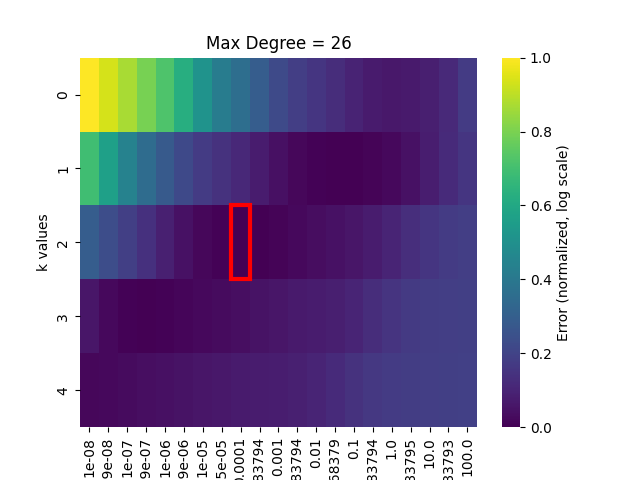
\includegraphics[width=0.72\textwidth]{figures/parameter_optimization_heatmap_L26.png}
    \caption{Five-fold cross-validated error surface over the regularisation strength $\lambda$ (x-axis) and Sobolev order $k$ (``k values'', y-axis) at fixed degree $L=26$. The selected minimum, $\lambda=10^{-4}$, $k=2$, is outlined in red.}
    \label{fig:heatmap}
\end{figure}

The heatmap shows how the cross-validated error changes with $\lambda$ and $k$ in \Cref{fig:heatmap}. The error decreases gradually when moving from $k=0$ (plain ridge-type regularisation) to $k=2$ (second-order Sobolev regularisation). This supports the idea that derivative-based regularisation is useful for the temperature reconstruction problem. $k=2$ provides stronger penalisation of high-degree and rough components, which helps reduce unnecessary high-frequency variation caused by noise. However, increasing $k$ too much can become overly restrictive. After $k=2$, the cross-validated error starts to increase again for larger $k$. This suggests that stronger smoothness penalties may begin to underfit genuine smaller-scale temperature variation. Therefore, the balance needs to be found where we cannot have either too little regularisation or too much. 

Although the heatmap does not show an extremely sharp minimum around $k=2$, the low-error region is relatively broad and shallow. This indicates that performance is not extremely sensitive to $k$ within the tested range, so the result aims to present some robustness choice of Sobolev order $k$. This finding is consistent with the predecessor dissertation that the second Sobolev seminorm could improve reconstruction compared with plain $L^2$ regularisation. Therefore, the current experiment provides an independent check using the temperature dataset and the current pipeline. Unless stated otherwise, the remaining experiments will use $L=26$, $\lambda=10^{-4}$, and $k=2$, which is selected from the grid search. The final configuration is then used in the subsequent conformal prediction experiments. 
 
\section{Standard versus adaptive coverage and width}
\label{sec:main-results}
\begin{table}[H]
\centering
\caption{Marginal coverage and mean interval width on the held-out test set ($n=351$, $\alpha=0.1$).}
\label{tab:main-coverage}
\begin{tabular}{lcc}
\toprule
Method & Marginal coverage & Mean interval width ($^\circ$C) \\
\midrule
Standard (non-adaptive) & 0.909 & 4.649 \\
Adaptive geodesic (proposed) & 0.937 & 4.592 \\
\bottomrule
\end{tabular}
\end{table}
The evaluation is performed on the held-out test set ($n=351$). The nominal conformal level ($\alpha=0.1$) corresponds to a target coverage of 90\%. The standard split conformal results show a marginal coverage of 90.9\% with a mean prediction interval width of $4.65^\circ\mathrm{C}$. In contrast, the proposed adaptive geodesic conformal results in a higher marginal coverage of 93.7\% with a mean prediction interval width of $4.59^\circ\mathrm{C}$ (\cref{tab:main-coverage}). Both approaches achieve the nominal 90\% coverage target on the held-out test set, which is consistent with the expected split-conformal coverage behaviour discussed in \cref{sec:cp-background} regardless of the spherical harmonic predictor used. However, the adaptive method provides higher coverage of 93.7\%, which is above the nominal 90\% target and slightly narrower mean prediction intervals. Besides, similar patterns can be seen across the different spherical harmonic degrees in the degree-robustness experiment \cref{tab:degree-robustness}. The variation across different $L$ values is also expected to align with finite-sample variation around the theoretical guarantee with $n_{cal}=351$. Overall marginal coverage alone is not the main reason for introducing the adaptive method. Since both methods already achieve approximately the desired overall coverage, the more important question is whether coverage remains reliable across locations with different prediction difficulties. Therefore, the next analysis focuses on conditional/difficulty-stratified coverage.
\begin{table}[H]
\centering
\caption{Conditional coverage and interval width by difficulty tertile (test set, $n=351$).}
\label{tab:tertile}
\begin{tabular}{lcccccc}
\toprule
Tertile & $n$ & $\overline{\hat\sigma}$ & $\overline{|e|}$ & Std.\ cov. & Adapt.\ cov. & Std.\ / Adapt.\ width \\
\midrule
Low difficulty & 118 & 0.310 & 0.366 & 1.000 & 0.915 & 4.649 / 1.481 \\
Medium difficulty & 117 & 0.815 & 0.820 & 0.957 & 0.949 & 4.649 / 3.893 \\
High difficulty & 116 & 1.770 & 1.904 & 0.767 & 0.948 & 4.649 / 8.460 \\
\bottomrule
\end{tabular}
\end{table}
The test set is split into three equal-frequency tertiles based on estimated local difficulty $\hat\sigma(x)$ to examine conditional/difficulty-dependent coverage, which cannot be seen from the overall marginal coverage (\cref{tab:tertile}). The standard method provides excessive coverage in the easiest tertile (100\% coverage above the 90\% target, with a fixed $4.65^\circ\mathrm{C}$ interval), while it demonstrates a sharp drop in the hardest tertile (76.7\% coverage, a 13.3 percentage-point gap below the target). These results show that the standard method does not maintain coverage consistently across different difficulty levels. In contrast, the adaptive method keeps coverage within a narrow $91$-$95\%$ range for all three difficulty groups, while obtaining a much narrower mean interval width of $1.48^\circ\mathrm{C}$ in the easiest tertile and a wider width of $8.46^\circ\mathrm{C}$ in the hardest tertile. This reflects that easier locations receive narrower intervals, while more difficult locations with greater uncertainty receive wider intervals. The hardest tertile also has a higher mean absolute prediction error of $1.90^\circ\mathrm{C}$, compared with the easiest tertile of $0.37^\circ\mathrm{C}$. This result shows that the adaptive method is responding to differences in local prediction difficulty and gives more balanced coverage across difficulty levels with varying interval widths according to local difficulty.
\begin{figure}[H]
    \centering
    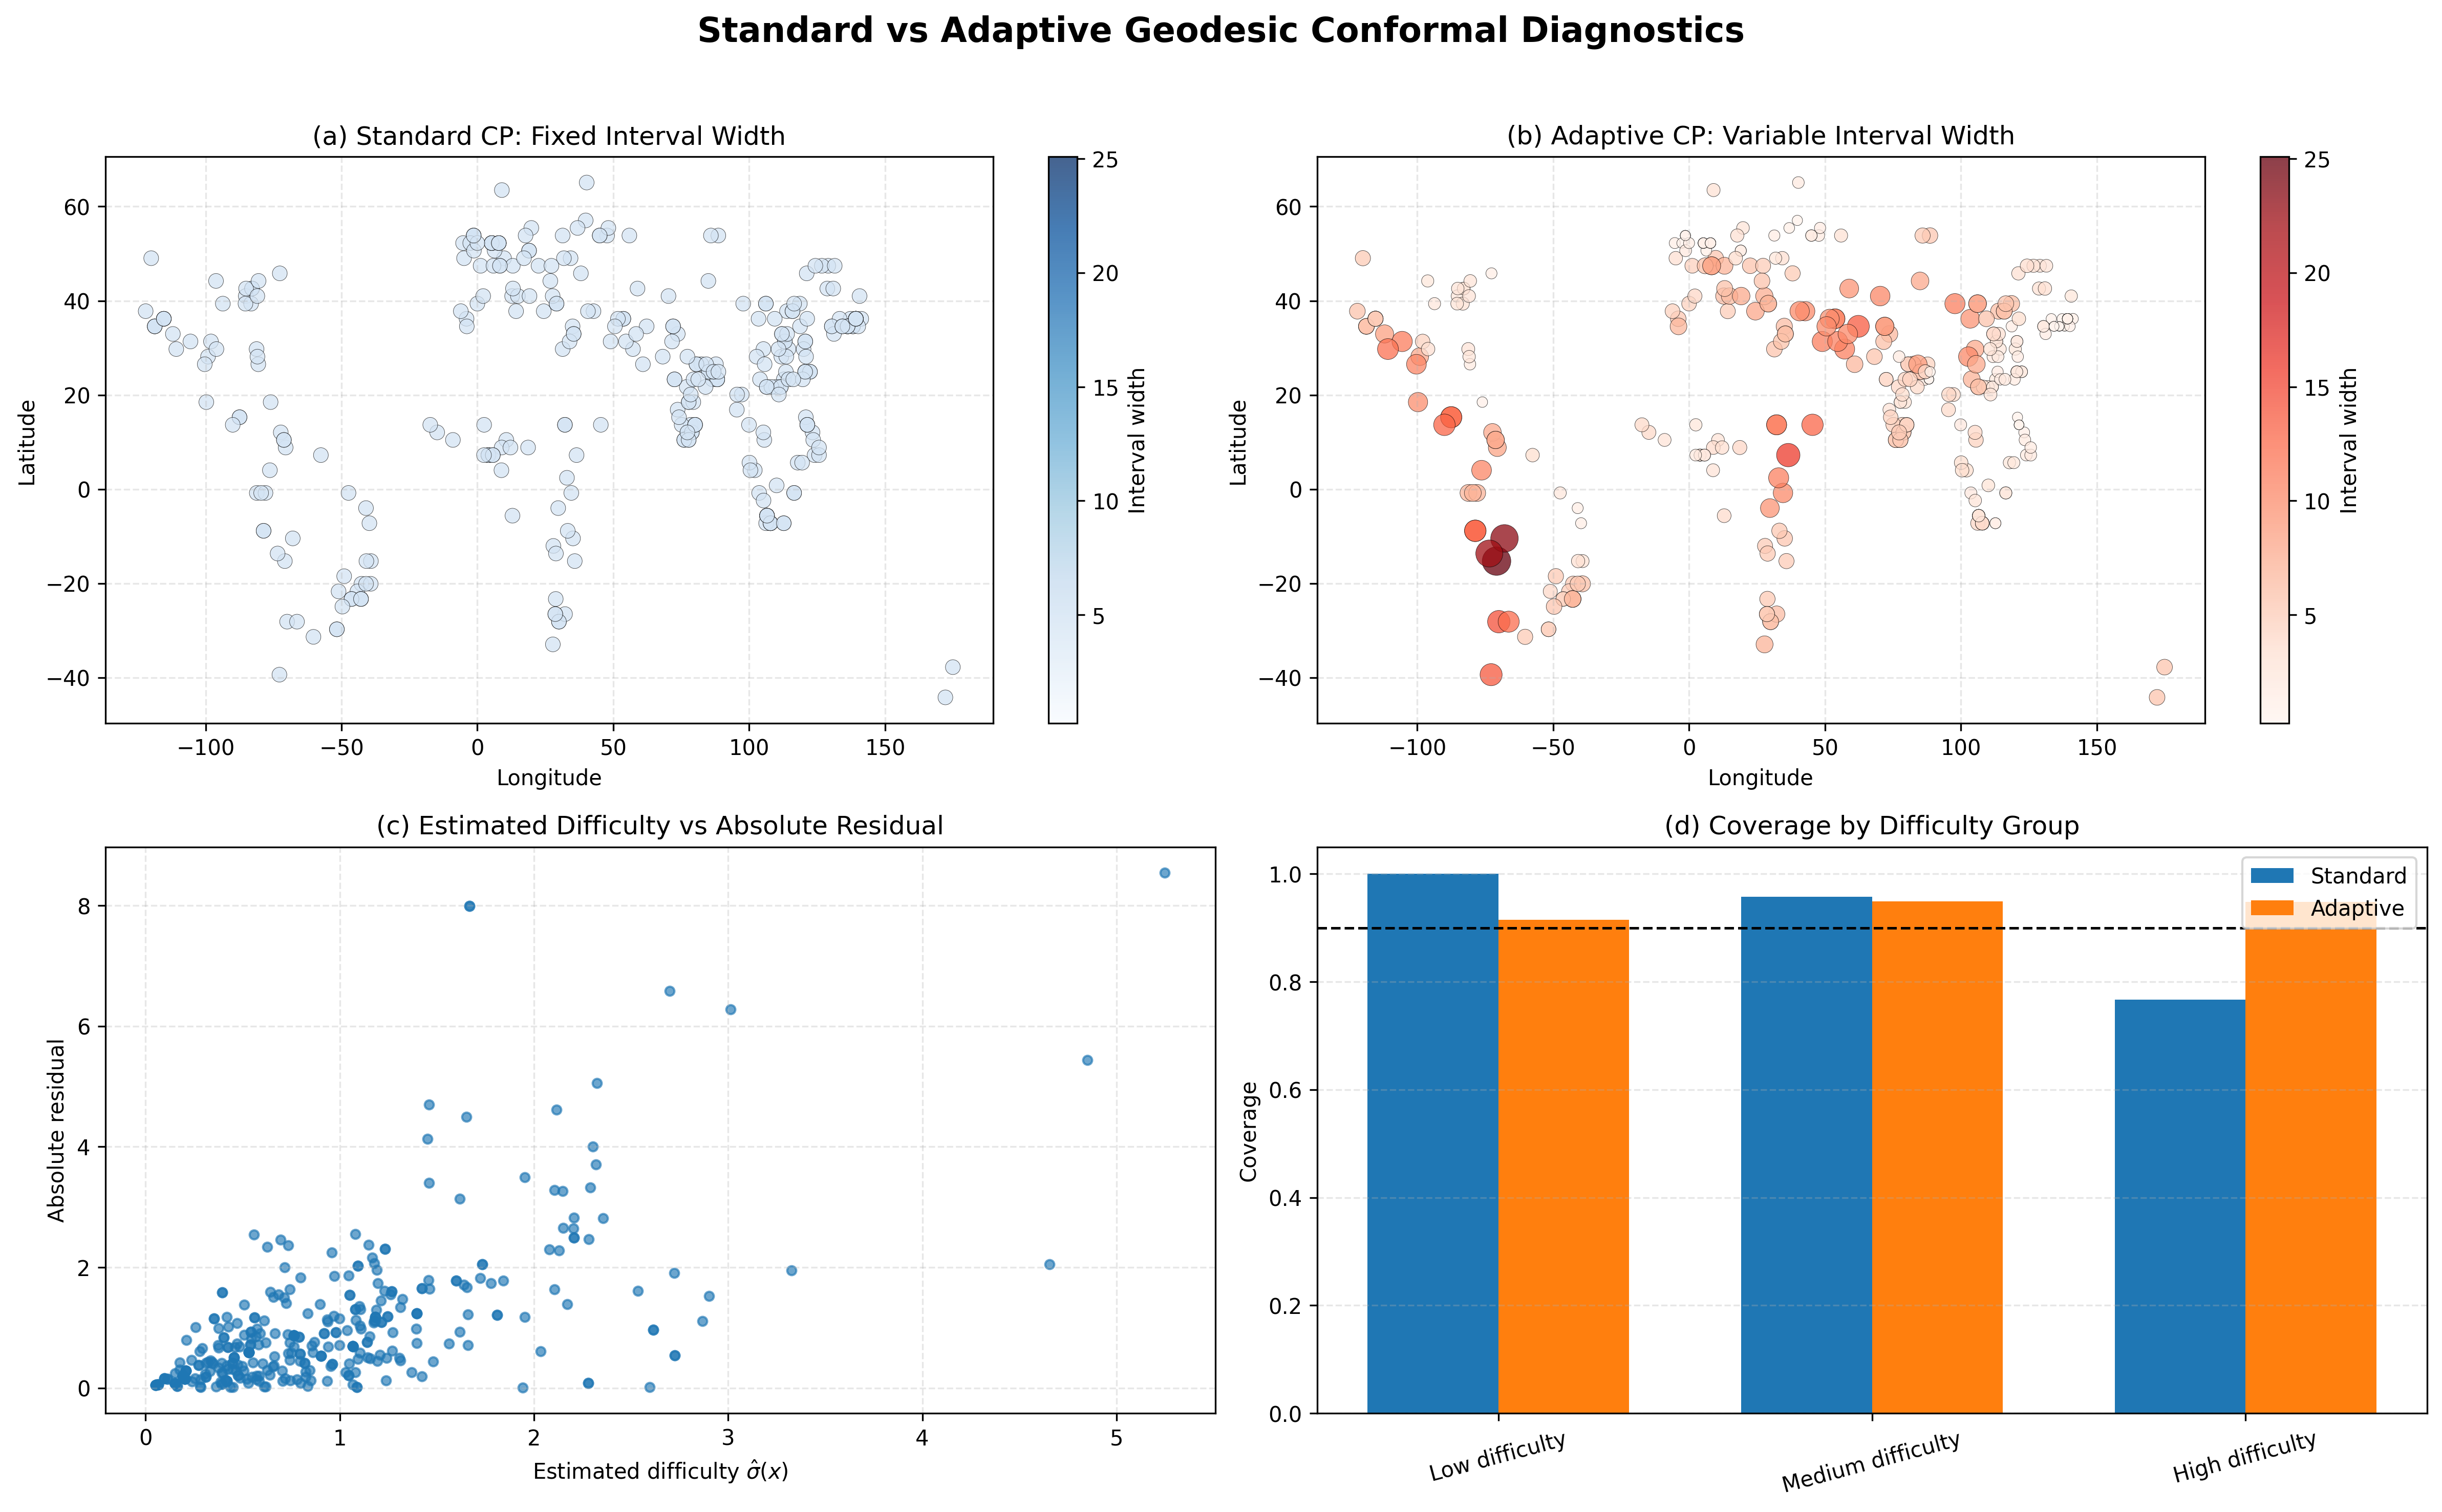
\includegraphics[width=\textwidth]{figures/standard_vs_adaptive_conformal_diagnostic.png}
    \caption{Standard versus adaptive geodesic conformal diagnostics on the test set. (a)/(b) Geographic distribution of interval width (marker size and colour) for the standard and adaptive methods. (c) Estimated difficulty $\hat\sigma(x)$ against true absolute residual. (d) Empirical coverage by difficulty tertile against the nominal $90\%$ target (dashed line).}
    \label{fig:main-diagnostic}
\end{figure}
\Cref{fig:main-diagnostic} presents the main result from both geographical and statistical perspectives. Panel (a) shows the spatial pattern of the standard conformal interval width, which is uniform across the spatial domain. Panel (b) shows that the adaptive method's interval widths vary across locations according to the estimated difficulty. Larger intervals are mainly found at high-difficulty locations, which are noticeably concentrated in western South America. Panel (c) shows a positive relationship between estimated difficulty $\hat\sigma(x)$ and the actual absolute prediction residual. Panel (d) gives the clearest single summary of the main result and visually demonstrates the difference in difficulty-stratified/conditional coverage: adaptive coverage (in orange) remains close to the 90\% target across all groups; standard coverage (in blue) varies between the groups.
\begin{figure}[H]
    \centering
        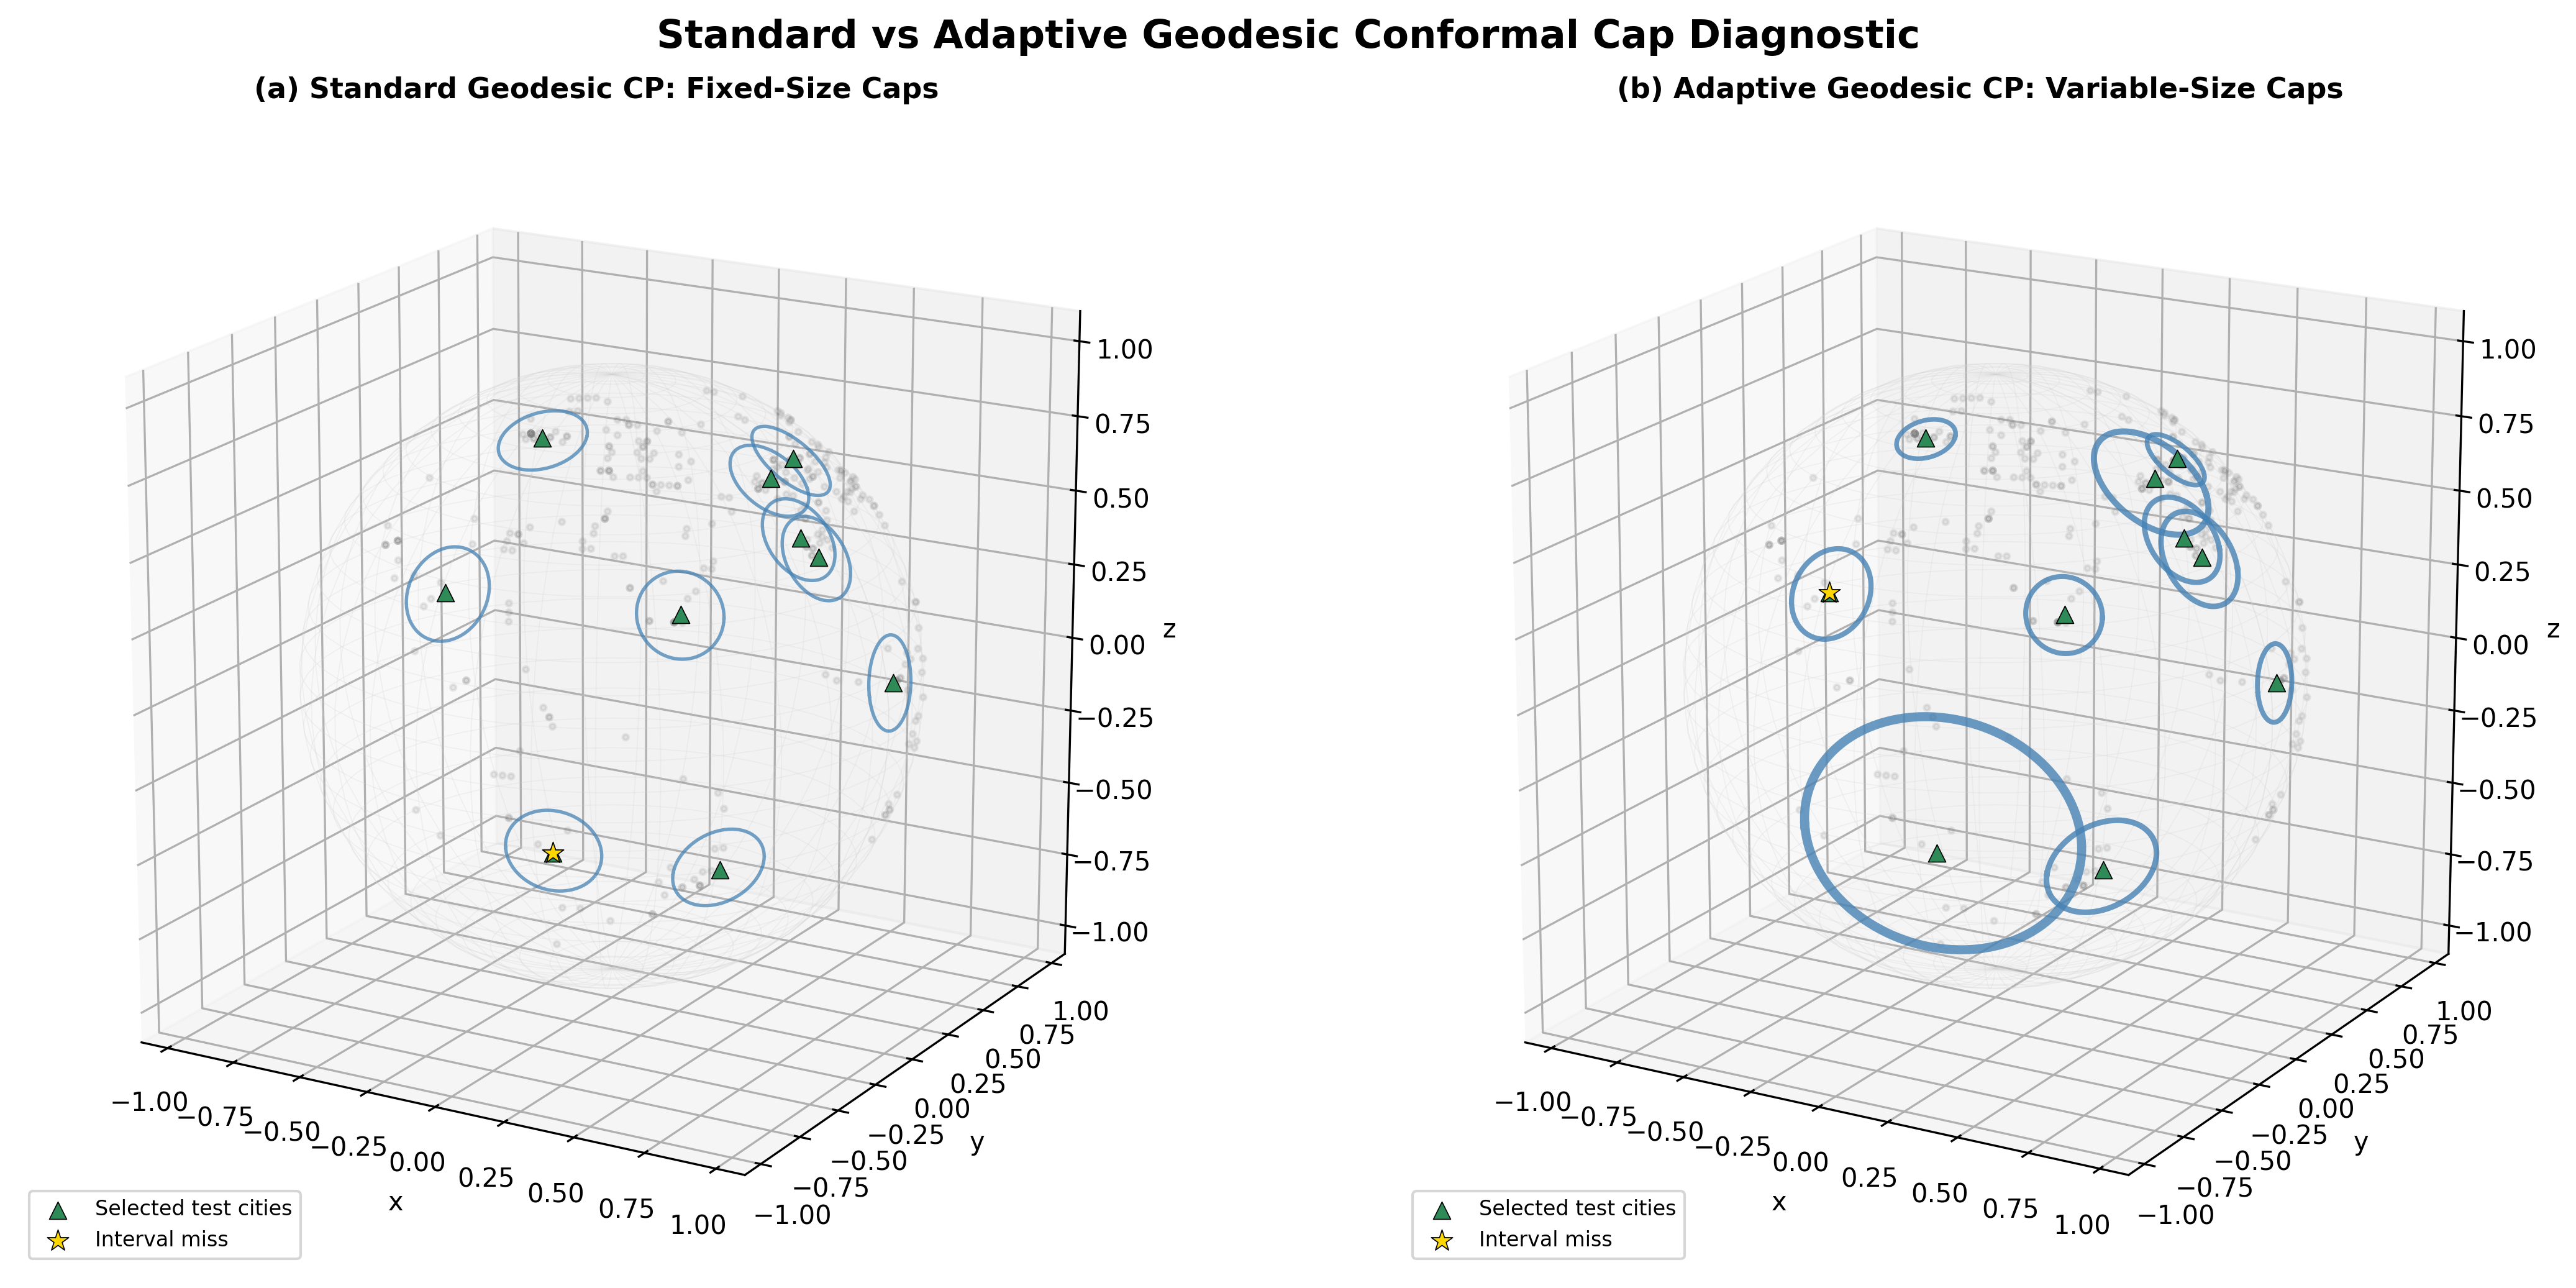
\includegraphics[width=\textwidth]{figures/standard_vs_adaptive_geodesic_caps.png}
    \caption{Illustrative fixed-size (standard, left) versus variable-size (adaptive, right) interval radii, drawn as circles on the input sphere for a representative subsample of test cities spanning the full difficulty range. Circle size is proportional to interval half-width; the gold star marks a coverage miss.}
    \label{fig:caps}
\end{figure}
\Cref{fig:caps} provides a geometric visualisation of the same adaptive uncertainty behaviour directly on the sphere. The standard conformal method uses the fixed-radius prediction caps, which do not change according to local difficulty. The adaptive method uses variable-radius caps, where larger caps are assigned to locations with higher estimated difficulty. The green triangles indicate the selected test cities, which are chosen to span the range of estimated prediction difficulty from low to high; the same locations are shown in both panels to allow a direct comparison between the standard and adaptive methods. The gold stars indicate test locations where the corresponding prediction cap does not contain the true value. In one example, the standard method's fixed and smaller cap does not cover the true value, while the adaptive method assigns a larger cap at the same location and successfully covers it. Conversely, another location is covered by the standard method but is missed by the adaptive method. These examples illustrate that adaptive conformal prediction does not eliminate individual misses, but instead reallocates interval width according to local prediction difficulty. The cap radii are visually rescaled rather than plotted using the raw values of $\hat q$ and $\hat q\hat\sigma(x)$, since these quantities are measured in temperature units, whereas the spherical cap radii are angular distances on the unit sphere. For visualisation, the adaptive interval widths are linearly mapped to spherical radii between $0.10$ and $0.45$, with smaller and larger radii corresponding to lower and higher estimated uncertainty, respectively. The standard method uses a single fixed visual radius, set to the median of the adaptive visual radii, to represent its constant interval width. The rescaling therefore preserves the relative differences in uncertainty while providing a meaningful geometric visualisation. Overall, the figure provides an intuitive geometric illustration of how adaptive interval widths respond to spatially varying prediction difficulty.

\section{Difficulty-estimator quality}
\begin{figure}[H]
    \centering
    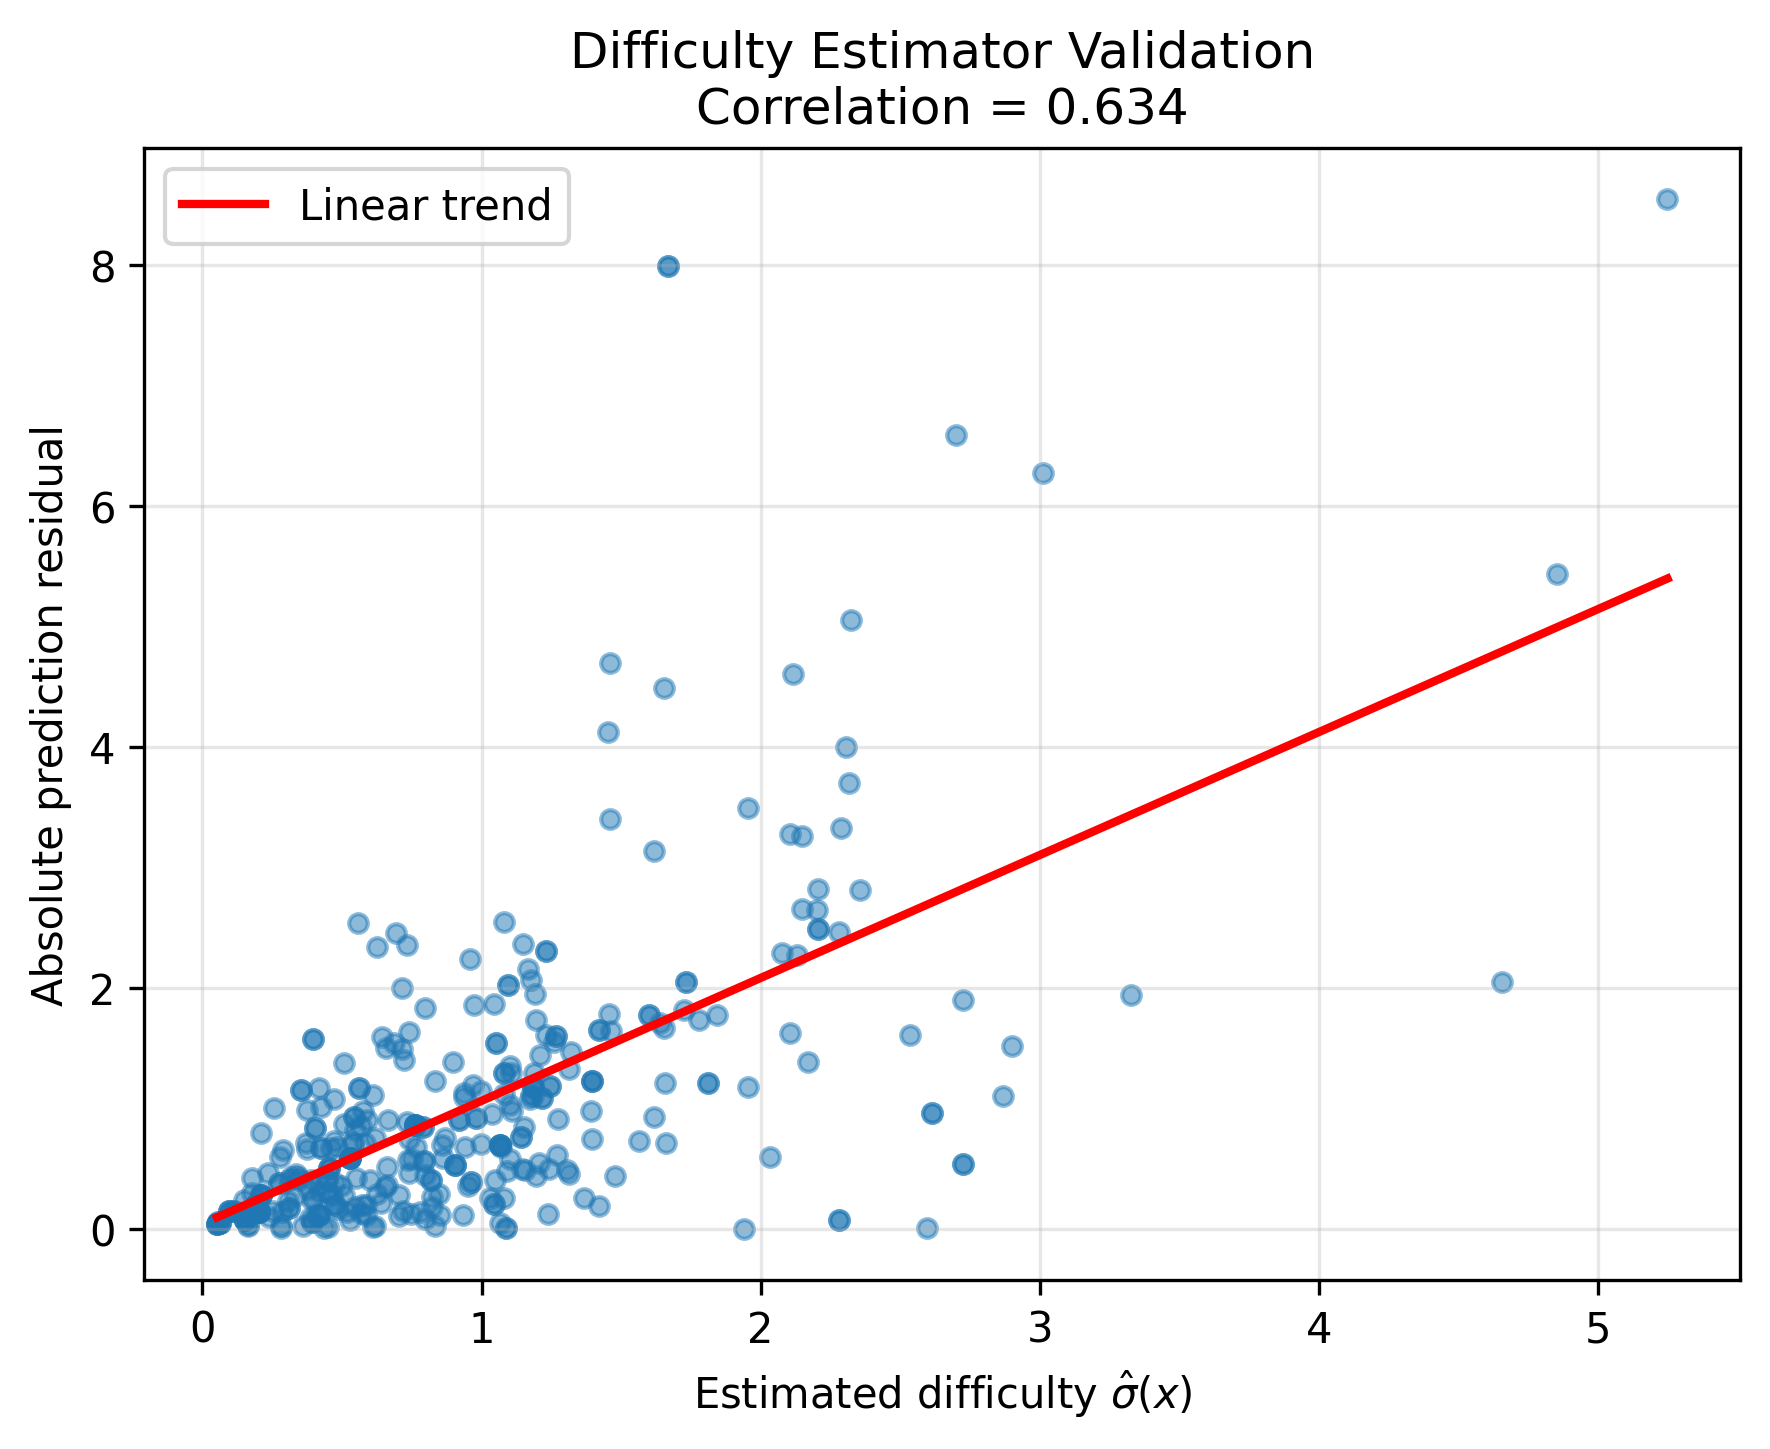
\includegraphics[width=0.65\textwidth]{figures/difficulty_validation.png}
    \caption{Estimated difficulty $\hat\sigma(x)$ against true absolute prediction residual on held-out data, with a linear trend line. Pearson $r=0.634$.}
    \label{fig:difficulty-validation}
\end{figure}
The Pearson correlation between the estimated difficulty $\hat\sigma(x)$ and the absolute prediction error on the held-out test set was $r=0.634$ (\cref{fig:difficulty-validation}). This indicates a clear positive relationship between the estimated local difficulty and the observed prediction error. Locations that are estimated to be more difficult generally tend to have larger prediction errors. The plot shows that $\hat\sigma(x)$ captures meaningful spatial variation in reconstruction difficulty. The current correlation result of $r=0.634$ is higher than the value reported by \citet{amirishahbazi2026} for their real-world IGRF-14 geomagnetic case study of $r=0.516$. Their experiments also found that correlations above approximately $0.3$ were associated with useful adaptive behaviour, however, this value should not be presented as a universal threshold. It should only be treated as an empirical reference from their experiments. 

With the current dataset, the result suggests that the geodesic $k$-nearest-neighbour residual estimator provides a useful measure of local reconstruction difficulty. Possible explanations for the difference from \citet{amirishahbazi2026}'s result are discussed in\cref{ch:discussion}. Correlation shows an empirical association but does not establish the physical cause of the relationship.

\section{Fine-grained conditional coverage}
\begin{table}[H]
\centering
\caption{Adaptive method conditional coverage across six equal-frequency difficulty bins (test set, $n=351$).}
\label{tab:sixbin}
\begin{tabular}{lccc}
\toprule
Bin & $n$ & Mean $\hat\sigma$ & Coverage \\
\midrule
1 (easiest) & 59 & 0.185 & 0.949 \\
2 & 59 & 0.435 & 0.881 \\
3 & 59 & 0.663 & 0.898 \\
4 & 58 & 0.969 & 1.000 \\
5 & 57 & 1.256 & 0.965 \\
6 (hardest) & 59 & 2.267 & 0.932 \\
\bottomrule
\end{tabular}
\end{table}
Instead of three difficulty tertiles, dividing the test set into six equal-frequency difficulty bins provides a more detailed assessment of how coverage changes across different levels of estimated difficulty and checks whether the adaptive method maintains stable coverage.  (\cref{tab:sixbin}). Coverage across the six bins ranges from $88.1\%$ to $100\%$, with a standard deviation of $0.0436$ and a worst-bin coverage of $88.1\%$. The worst bin is therefore $1.9$ percentage points below the nominal $90\%$ target. This indicates that the adaptive method maintains relatively stable coverage across the different levels, with no difficulty bin showing a very large departure from the target coverage. Thus, the adaptive method provides more consistent conditional coverage across locations with different difficulty levels, with its worst six-bin coverage of 88.1\% also being higher than the 76.7\% coverage observed in the worst tertile for the standard method (\cref{tab:tertile}). Overall, the six-bin analysis provides additional evidence that the adaptive method is not only achieving good marginal coverage but also maintaining relatively stable coverage across different difficulty levels.

\section{Robustness across spherical harmonic degree}
\begin{figure}[H]
    \centering
    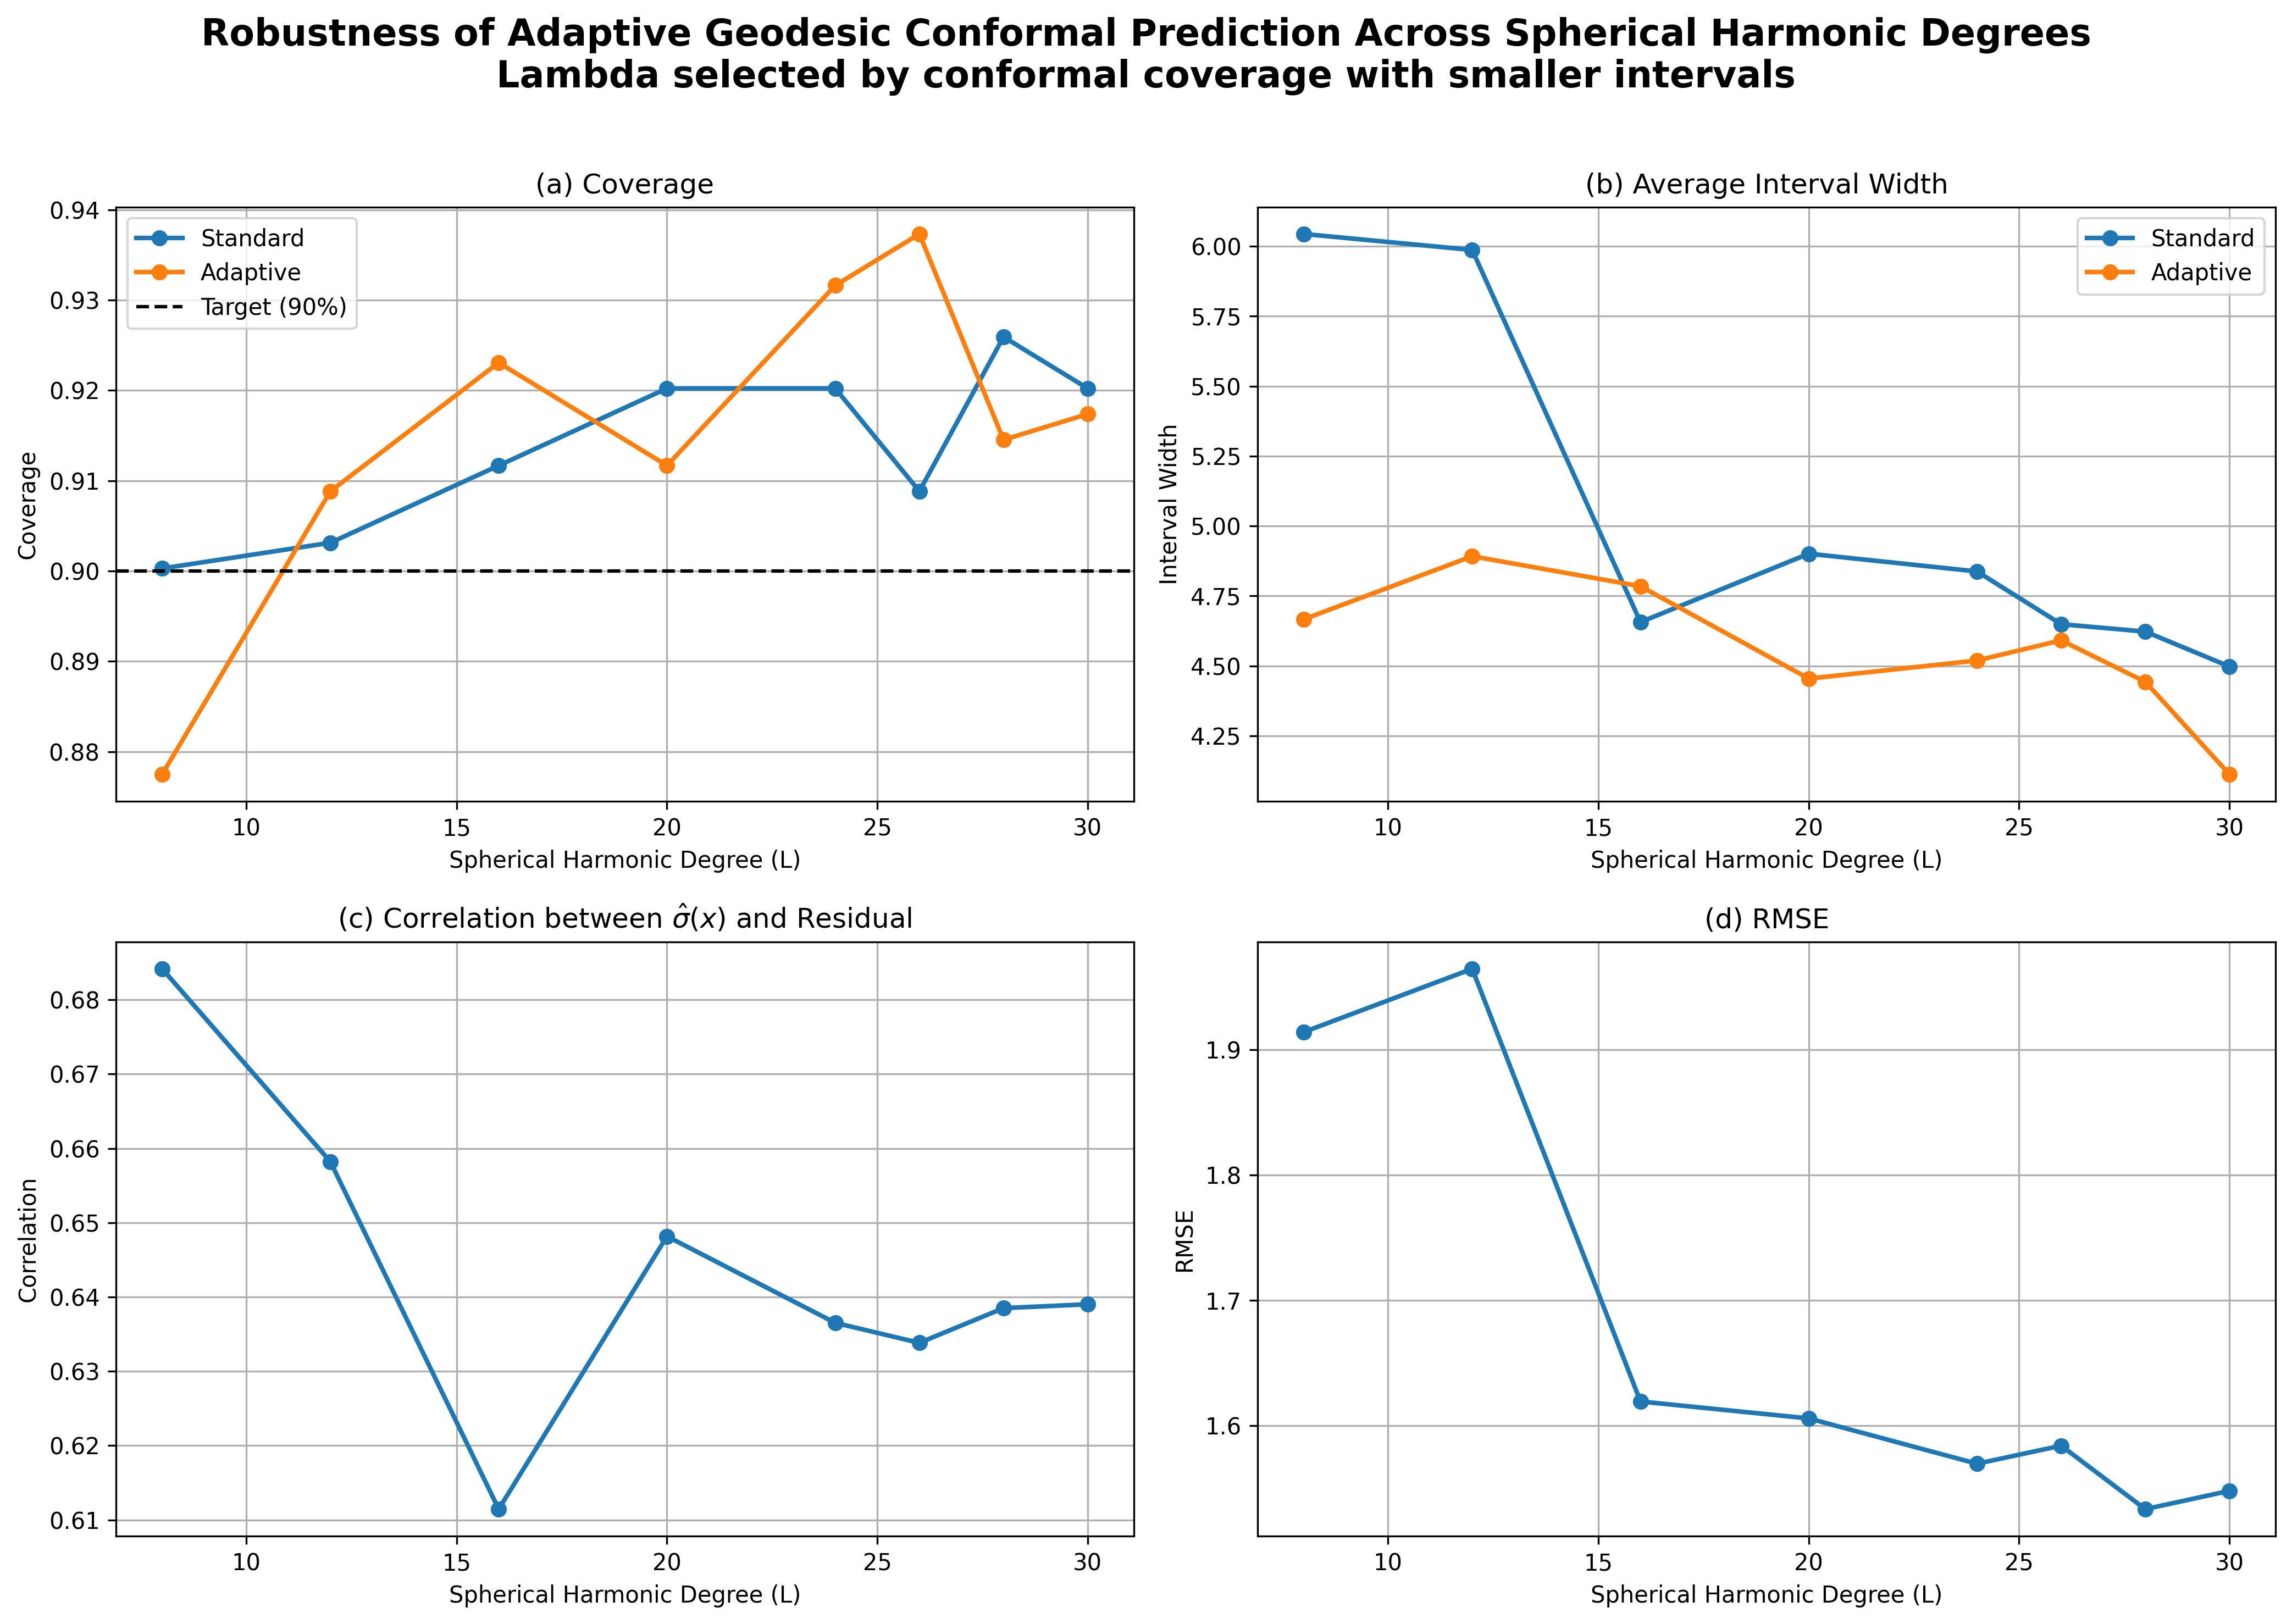
\includegraphics[width=\textwidth]{figures/degree_robustness_conformal_lambda_summary.png}
    \caption{Robustness of adaptive geodesic conformal prediction across spherical harmonic degree $L$, with $\lambda$ selected to minimise adaptive interval width subject to a $90\%$ validation-coverage constraint. (a) Coverage. (b) Mean interval width. (c) Correlation between $\hat\sigma(x)$ and true residual. (d) Test RMSE.}
    \label{fig:degree-robustness}
\end{figure}
To assess whether the main results in  \cref{sec:main-results} depend strongly on the specific degree $L=26$, the full pipeline was repeated for $L\in\{8,12,16,20,24,26,28,30\}$. At each degree, $\lambda$ is re-selected using both the RMSE-minimising and conformal-efficiency criteria described in \cref{ch:methodology}. \Cref{fig:degree-robustness} shows the results for the conformal-selected $\lambda$. Adaptive coverage (panel (a)) stays reasonably close to the $90\%$ target across the tested degrees, while adaptive interval width (panel (b)) is generally similar or below the standard interval width, except for $L\geq20$, which suggests that adaptive uncertainty does not require substantially wider intervals at higher levels of model complexity. The difficulty-estimator correlation $r$ (panel (c)) is highest at the lowest degree tested ($r=0.684$ at $L=8$) and settles into a relatively stable range of approximately $0.63$-$0.66$ for $L\geq20$, suggesting that the relationship between estimated difficulty and actual prediction error remains reasonably stable across higher model degrees. Test RMSE (panel (d)) shows an overall decrease as the degree increases, with only a small increase from $L=8$ to $L=12$, before decreasing substantially from $L=12$ to $L=16$ and then slowly decreasing towards $L=30$. The results suggest that the improvements become smaller and somewhat non-monotonic beyond $L=24$, indicating a gradual reduction in the benefit of additional model complexity. Overall, the adaptive conformal method remains reasonably stable across different spherical harmonic degrees. Increasing model complexity generally improves reconstruction accuracy, but the benefit becomes smaller at higher degrees. The uncertainty results do not appear to depend strongly on selecting exactly $L=26$. This provides evidence of robustness to the choice of spherical harmonic model complexity.
\begin{table}[H]
\centering
\caption{Degree-robustness results with $\lambda$ selected by conformal efficiency (minimum adaptive width subject to $\ge 90\%$ validation coverage). ``Std.\ cov.'' / ``Adapt.\ cov.'' are test-set marginal coverage; $r$ is the difficulty-estimator correlation; $\sigma_{\mathrm{cond}}$ is the six-bin conditional coverage standard deviation; ``Worst'' is the worst-bin coverage.}
\label{tab:degree-robustness}

\resizebox{\textwidth}{!}{%
\begin{tabular}{lccccccccc}
\toprule
$L$ & $\lambda$ & Std.\ cov. & Adapt.\ cov. & Std.\ width & Adapt.\ width & $r$ & $\sigma_{\mathrm{cond}}$ & Worst & RMSE \\
\midrule
8  & $3.16\times10^{-6}$ & 0.900 & 0.877 & 6.044 & 4.667 & 0.684 & 0.036 & 0.828 & 1.914 \\
12 & $1.00\times10^{-2}$ & 0.903 & 0.909 & 5.987 & 4.892 & 0.658 & 0.043 & 0.867 & 1.965 \\
16 & $1.00\times10^{-6}$ & 0.912 & 0.923 & 4.657 & 4.785 & 0.611 & 0.034 & 0.891 & 1.619 \\
20 & $1.00\times10^{-4}$ & 0.920 & 0.912 & 4.901 & 4.455 & 0.648 & 0.036 & 0.864 & 1.606 \\
24 & $3.16\times10^{-5}$ & 0.920 & 0.932 & 4.838 & 4.520 & 0.637 & 0.034 & 0.897 & 1.570 \\
26 & $1.00\times10^{-4}$ & 0.909 & 0.937 & 4.649 & 4.592 & 0.634 & 0.044 & 0.881 & 1.584 \\
28 & $3.16\times10^{-4}$ & 0.926 & 0.915 & 4.623 & 4.443 & 0.638 & 0.044 & 0.847 & 1.533 \\
30 & $3.16\times10^{-5}$ & 0.920 & 0.917 & 4.498 & 4.113 & 0.639 & 0.051 & 0.852 & 1.548 \\
\bottomrule
\end{tabular}%
}
\end{table}
\Cref{tab:degree-robustness}  lists the detailed results for the conformal-selected $\lambda$ at each spherical harmonic degree, including the six-bin conditional-coverage standard deviation and worst-bin coverage. The conditional coverage standard deviation remains within $0.033$ to $0.051$ across all tested degrees, whereas the worst-bin coverage ranges from $0.828$ to $0.897$. Conditional coverage does vary a little across model degrees, yet the overall behaviour remains quite good. These results suggest that the advantage of the adaptive method over the standard baseline in \cref{sec:main-results} at $L=26$ can also be observed across other spherical harmonic degrees.

The marginal-coverage columns of \cref{tab:degree-robustness} assess how stable the conformal calibration is when the model complexity changes. For the eight degrees tested, standard conformal marginal coverage ranges from $90\%$ to $92.6\%$, while adaptive conformal marginal coverage ranges from $87.7\%$ to $93.7\%$. Only at $L=8$ is adaptive coverage slightly below the nominal 90\% target, while at the other tested degrees, it stays reasonably close to $90\%$.  This indicates that the calibration procedure remains broadly stable as the spherical harmonic degree changes, with some variation expected because of finite test/calibration sample sizes.

The test RMSE from 1.914 at $L=8$ drops to approximately 1.53-1.55 for $L=28$, indicating that the accuracy of the base model improves. However, the improvement becomes smaller when the degree becomes higher, which suggests a diminishing benefit from adding further model complexity. Also, the correlation and conditional coverage remain relatively stable across all tested degrees. So, the main findings are not strongly affected by the choice of $L$.
\begin{figure}[H]
    \centering
    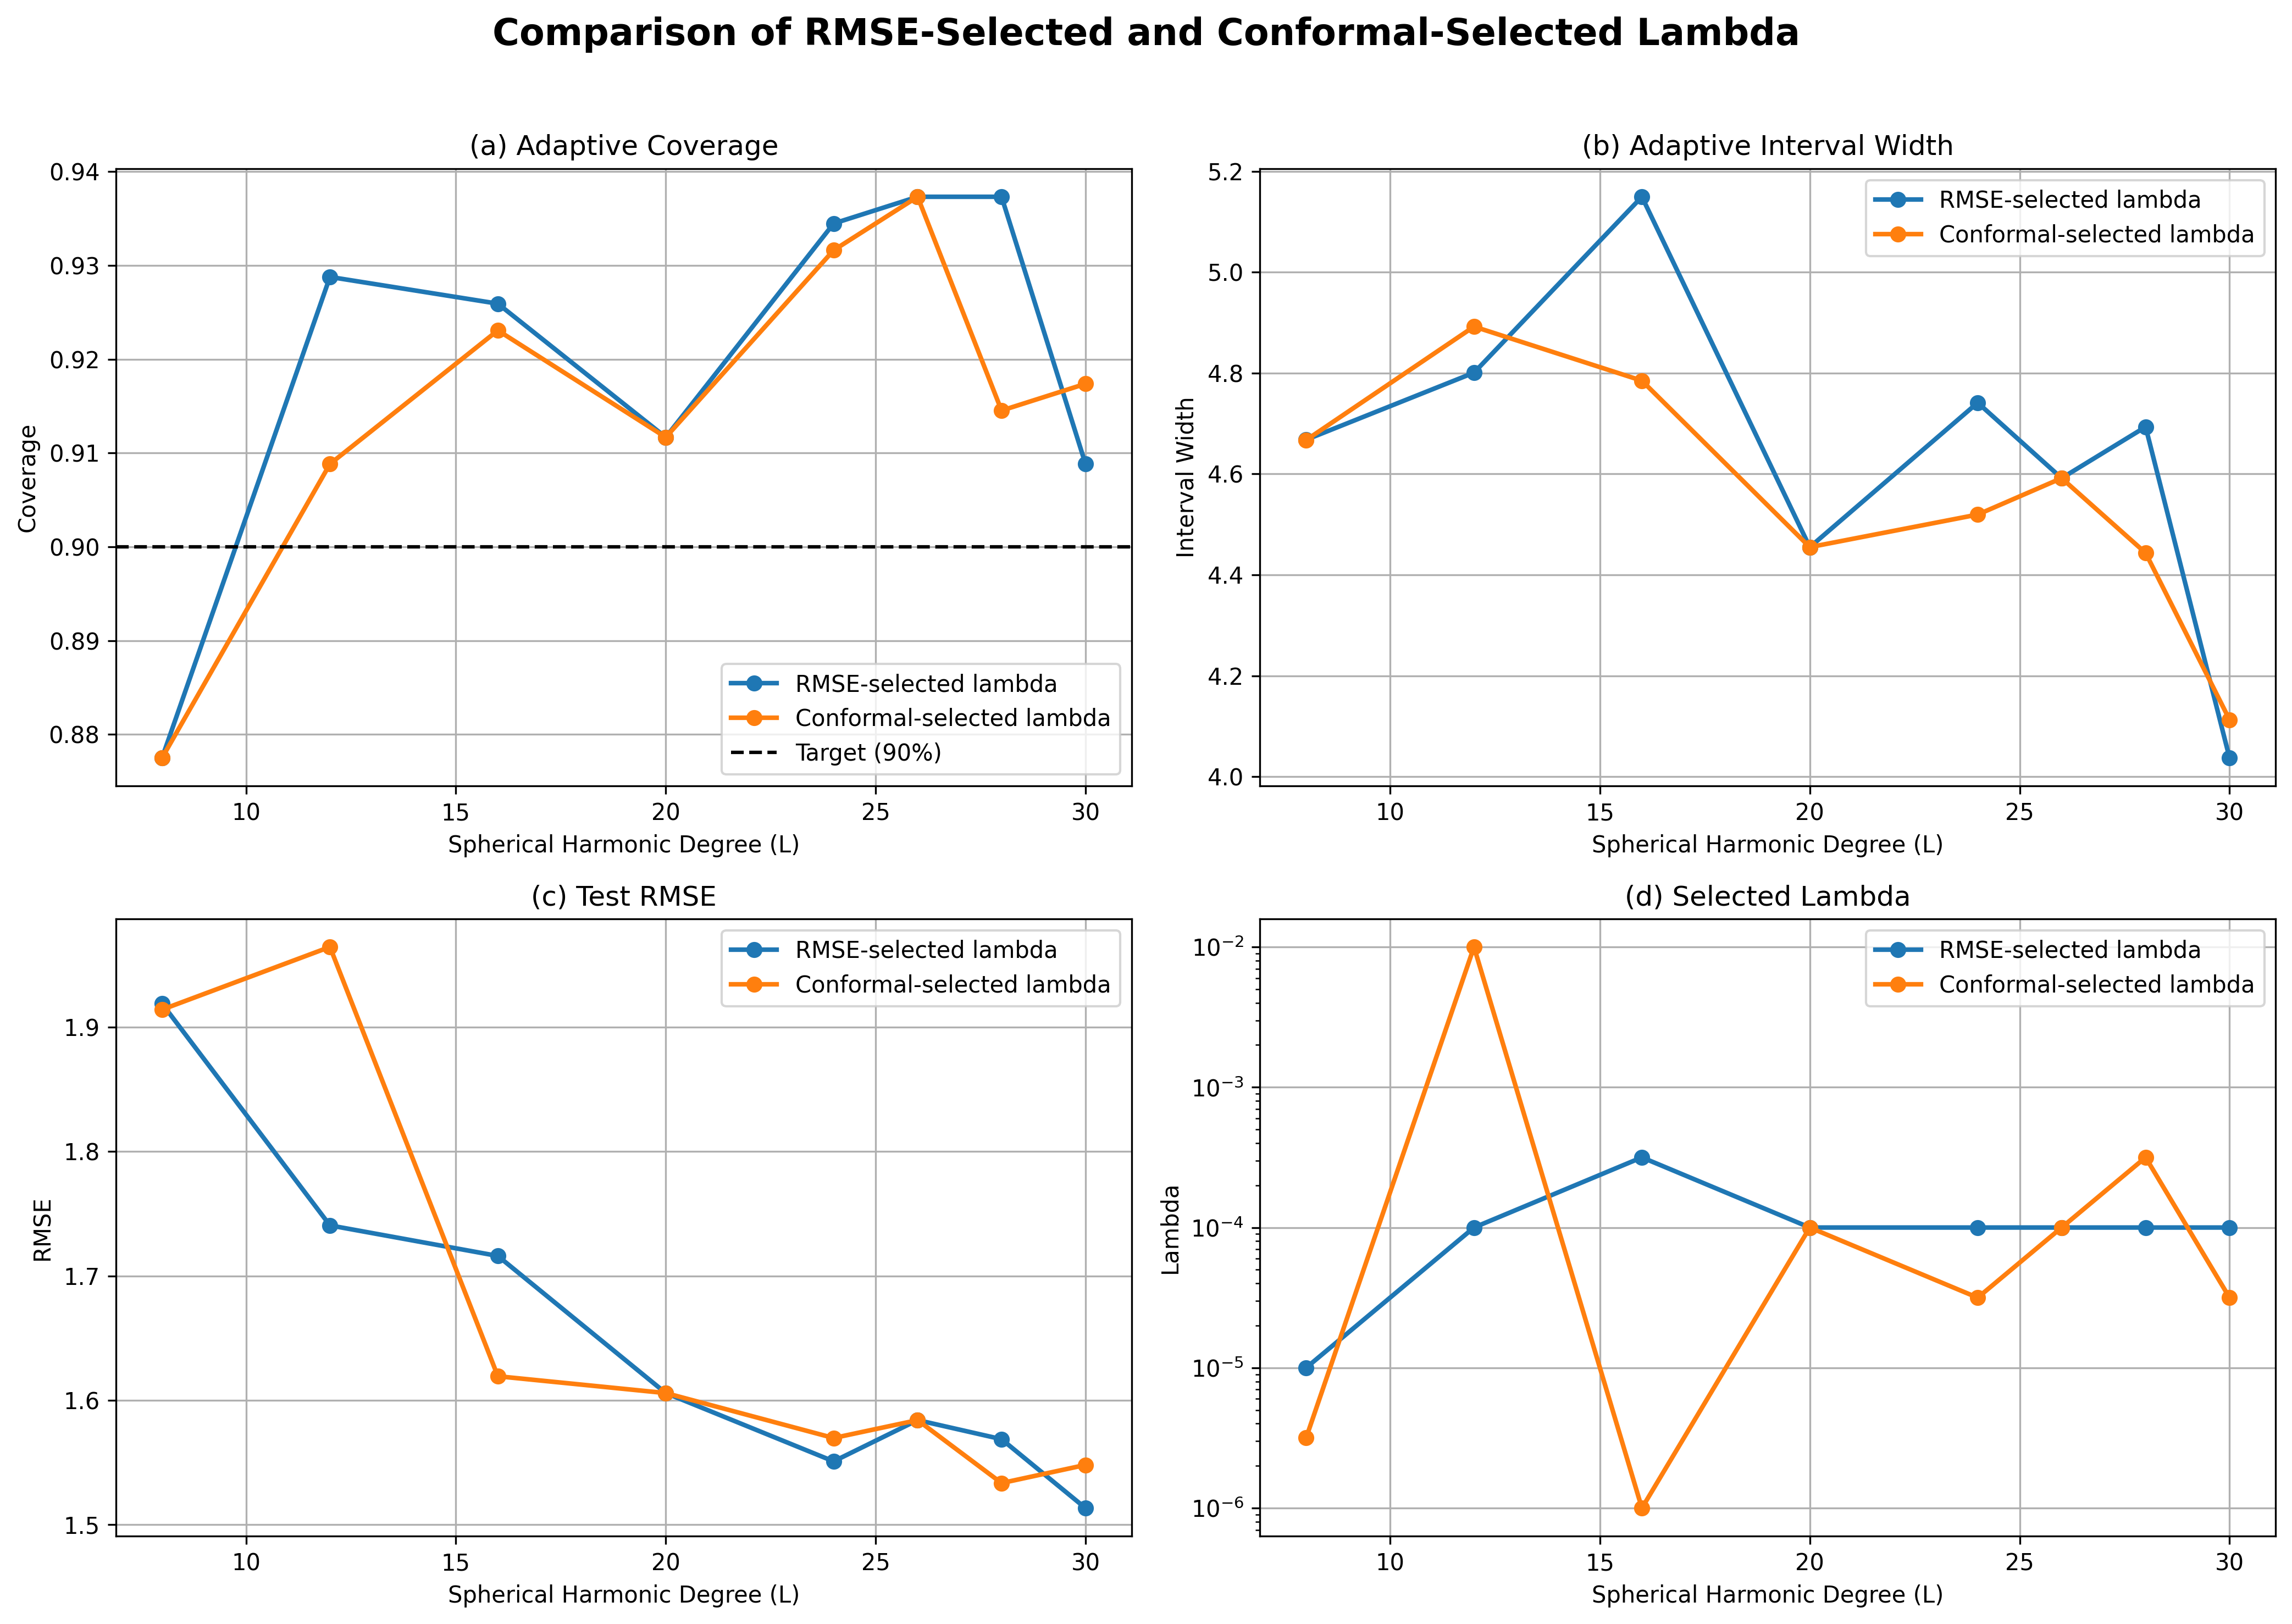
\includegraphics[width=\textwidth]{figures/degree_robustness_lambda_comparison_summary.png}
    \caption{Comparison of RMSE-selected and conformal-efficiency-selected regularisation strength $\lambda$ across spherical harmonic degree.}
    \label{fig:lambda-comparison}
\end{figure}
\Cref{fig:lambda-comparison} compares two different criteria for selecting $\lambda$: RMSE-based selection, which prioritises prediction accuracy, and conformal-based selection, which prioritises interval efficiency while satisfying the coverage requirement. Overall, both methods are consistent in direction for adaptive coverage, interval width, and test RMSE except for the $\lambda$ results in panel (d). For example, at $L=12$, the RMSE-selected $\lambda=10^{-4}$, while the conformal-selected $\lambda=10^{-2}$. This suggests that changing the selection criterion does not appear to cause a large change in overall performance, but the selected $\lambda$ changes depending on the objective being prioritised. Prediction accuracy and conformal interval efficiency appear to be positively correlated in this experiment. However, this should be treated as an empirical observation but not a theoretical guarantee. The two criteria focus on different objectives. A $\lambda$ value that gives the lowest RMSE may not produce the narrowest conformal intervals while still maintaining the required coverage. Therefore, the similar results observed here do not mean that the two selection approaches will always produce the same results.

\section{Full-field reconstruction and geographic uncertainty}
\label{sec:geography}
\begin{figure}[H]
    \centering
    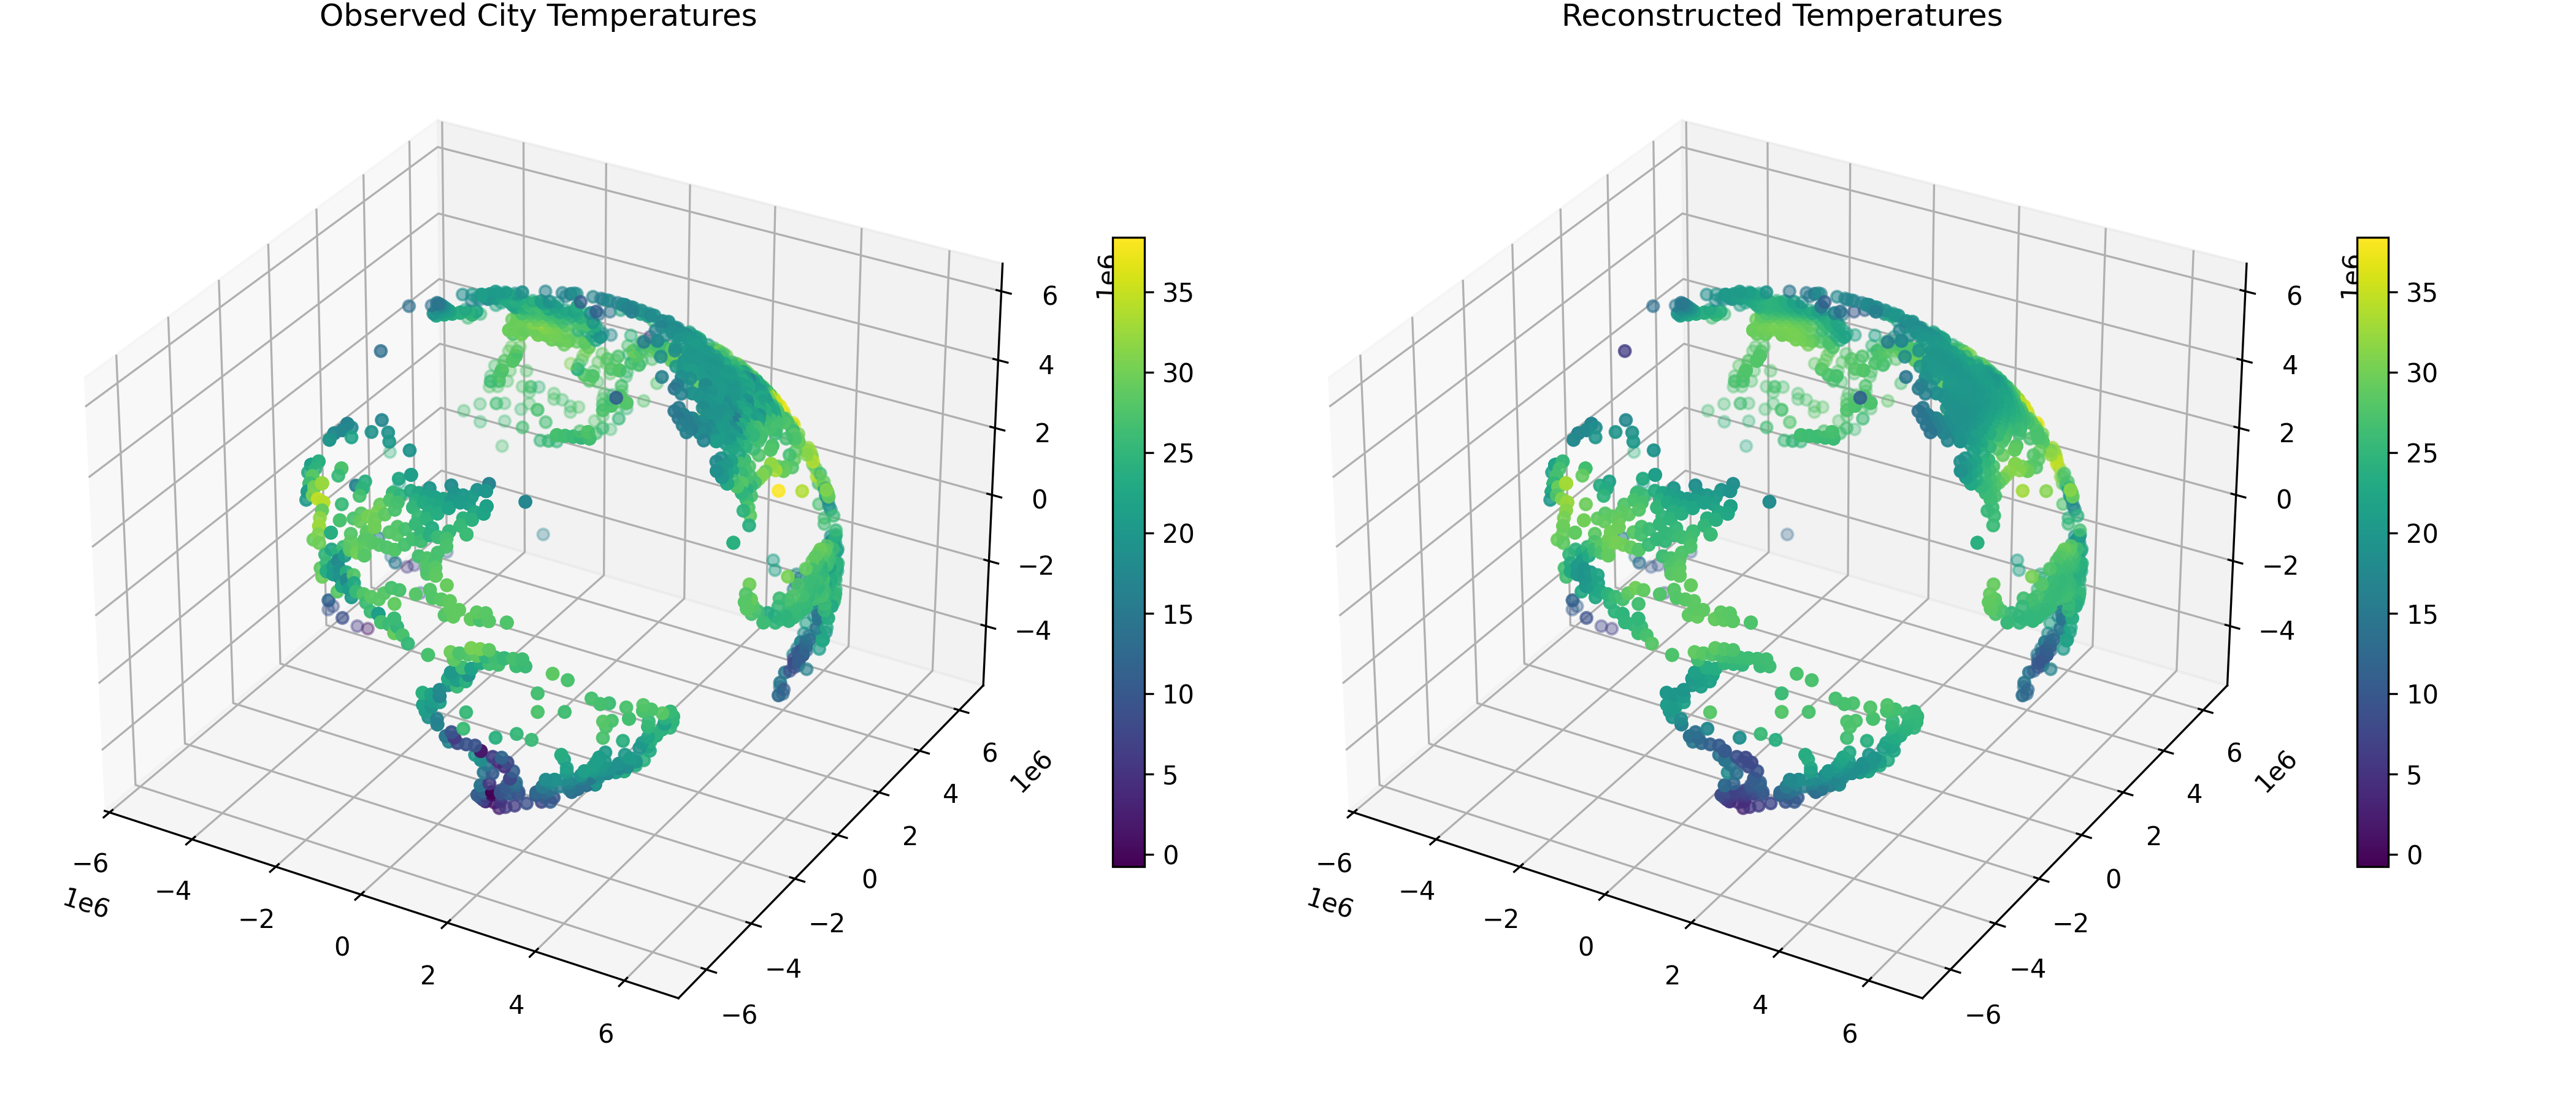
\includegraphics[width=\textwidth]{figures/observed_vs_reconstructed.png}
    \caption{Observed (left) and reconstructed (right) city temperatures, plotted on a 3D globe of Earth's radius. Both use the same colour scale.}
    \label{fig:reconstructed}
\end{figure}
The calibrated model ($L=26$, $\lambda=10^{-4}$, $k=2$) is used to reconstruct the temperature field on a dense $50\times50$ evaluation grid covering the whole sphere. It is also evaluated separately at all $3{,}510$ city locations, giving an overall reconstruction $\mathrm{RMSE}=1.442^\circ\mathrm{C}$, $\mathrm{MAE}=0.921^\circ\mathrm{C}$, and bias $-0.004^\circ\mathrm{C}$. These values indicate the reconstructed temperatures are generally close to the observed temperatures. The evaluation includes training points, and thus it reflects the overall reconstruction fit. They should not be interpreted as out-of-sample performance. The out-of-sample accuracy is evaluated separately using the held-out test set in \cref{sec:main-results}. \Cref{fig:reconstructed} compares the observed and reconstructed temperature fields. The reconstruction captures the main latitudinal patterns and the continental patterns in the observed data. This suggests that the spherical harmonic model successfully captures the large-scale structure of the observed temperature field.
\begin{figure}[H]
    \centering
    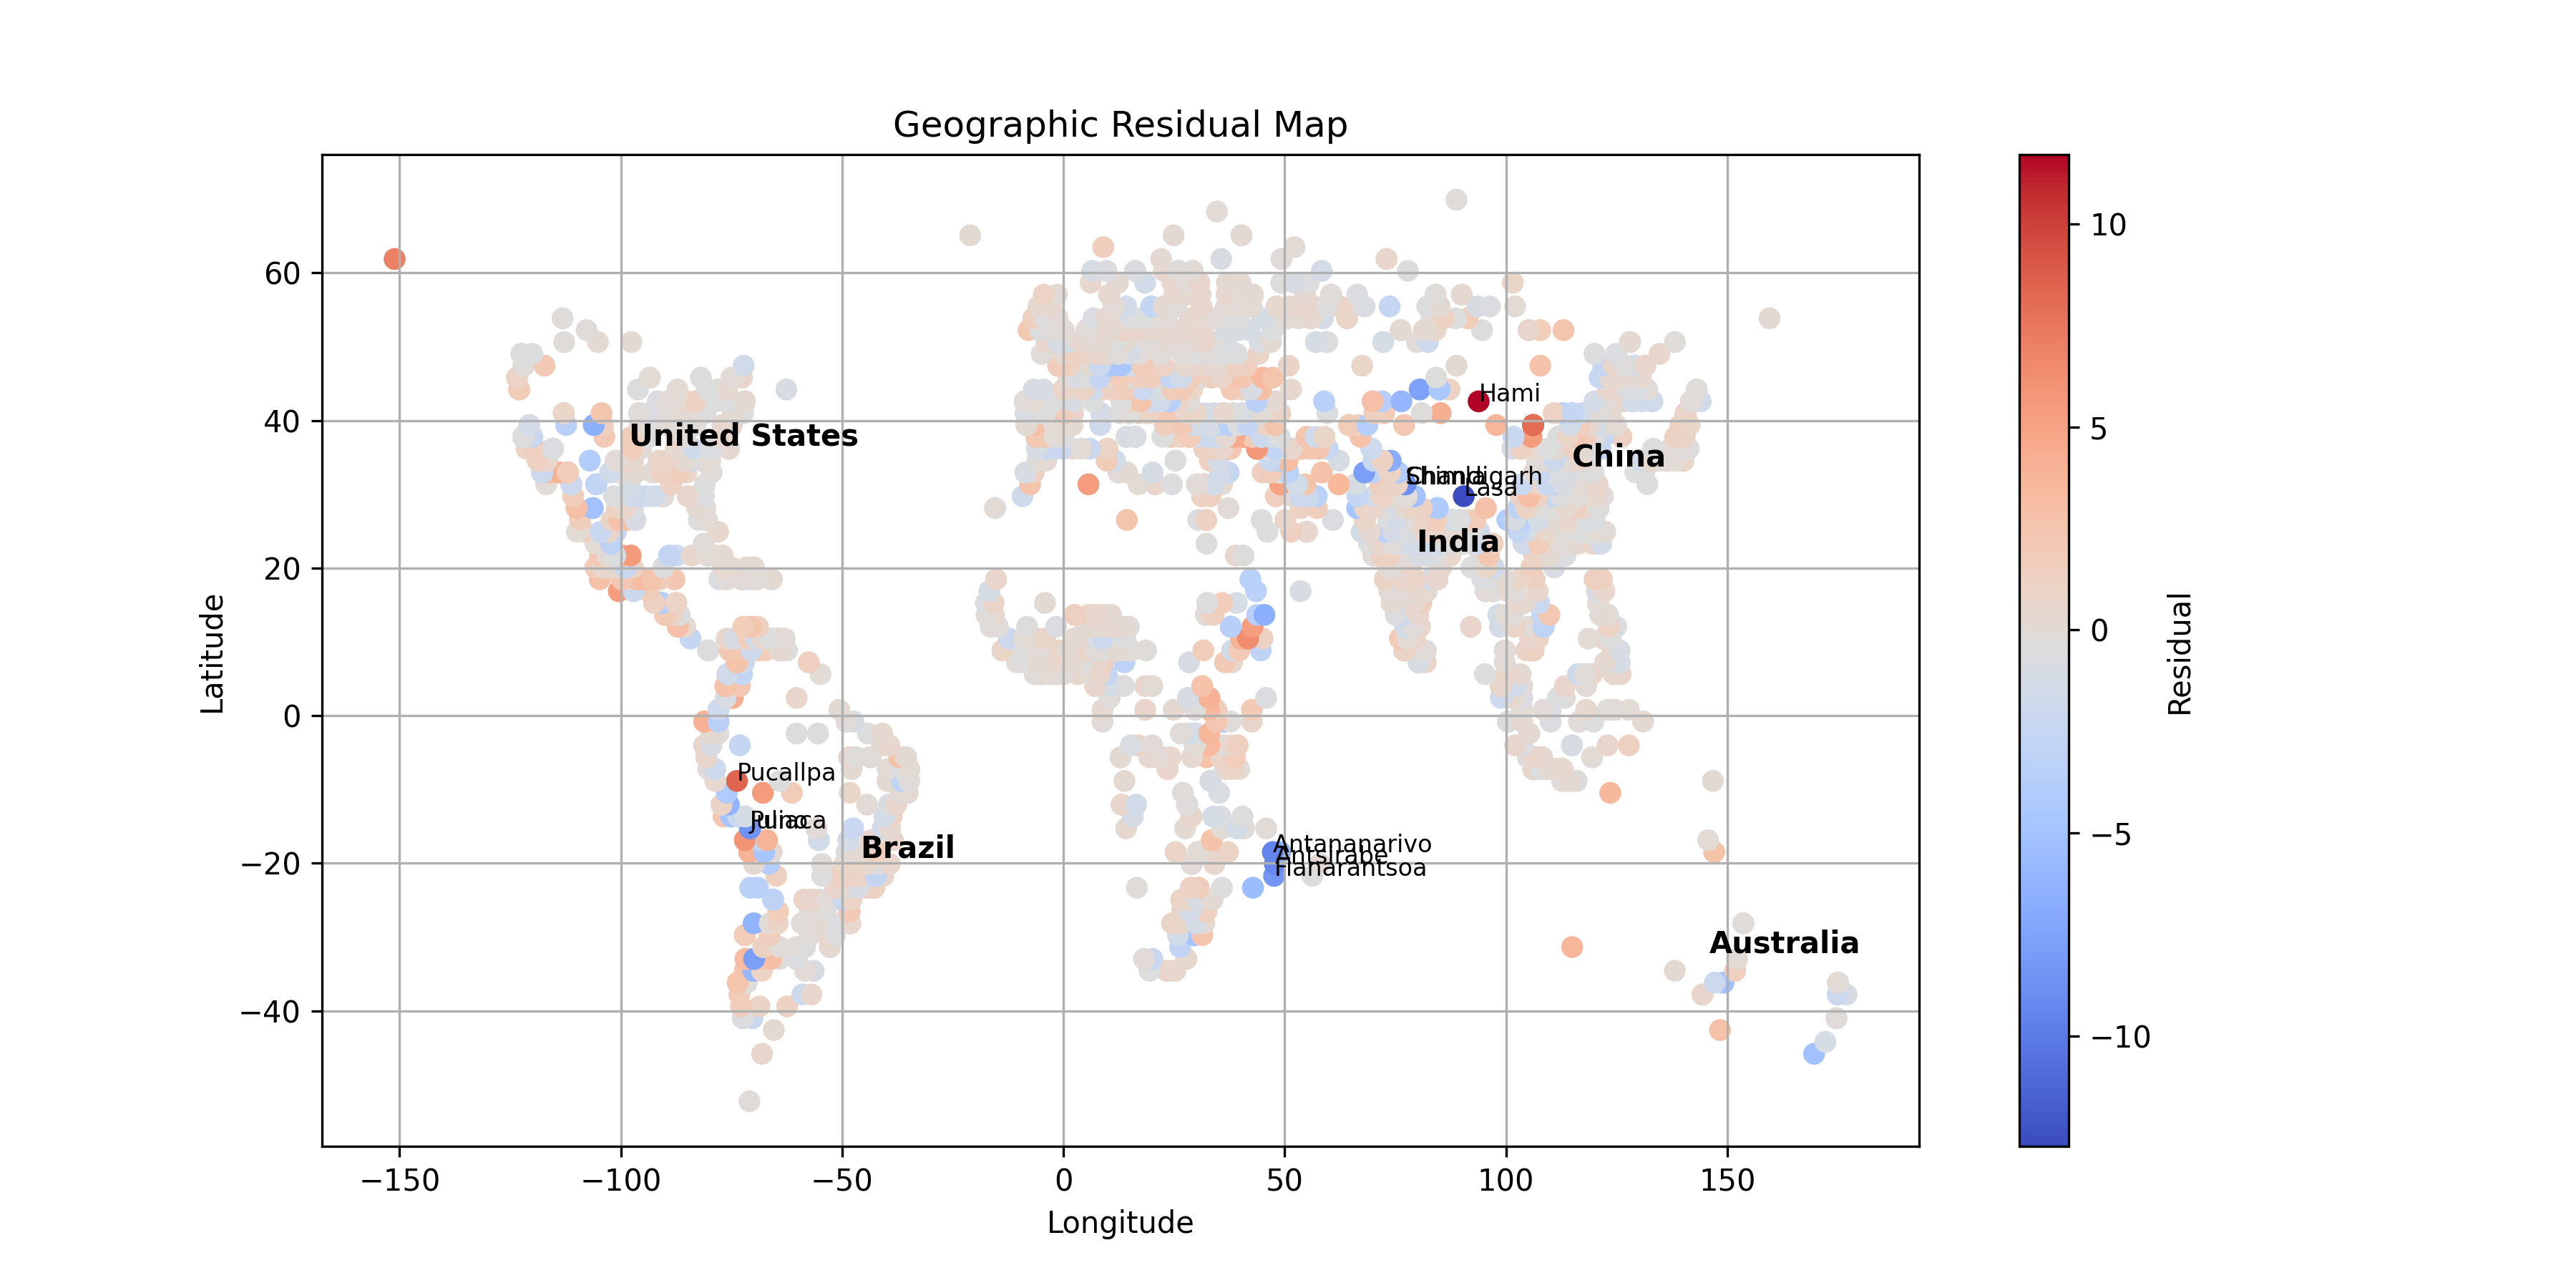
\includegraphics[width=\textwidth]{figures/geographic_residual_map.png}
    \caption{Geographic distribution of signed reconstruction residuals (observed minus predicted), with the ten largest-magnitude residual cities and several major-country centroids labelled for orientation.}
    \label{fig:geo-residual}
\end{figure}
The residual field (\cref{fig:geo-residual}) shows the geographic distribution of reconstruction residuals. No obvious large-scale systematic geographic pattern is observed here, and the residuals are relatively small for most locations. The overall reconstruction bias reported above ($-0.004^\circ\mathrm{C}$) is negligible relative to the overall variation in global city temperatures. However, a small number of cities have noticeably larger residuals in both directions. For instance, Hami, China, is over-predicted, while several Himalayan-region stations are under-predicted. These larger residuals may be related to local climatic characteristics, such as extreme continental conditions, high-altitude environments, or other local effects. These local variations may be difficult for a smooth spherical harmonic model to represent accurately. At $L=26$, the nominal angular scale associated with the maximum degree is approximately $180^\circ/L \approx 7^\circ$, limiting the model's ability to represent highly localised spatial variation. This might be one reason for some of the larger local residuals.
\begin{figure}[H]
    \centering
    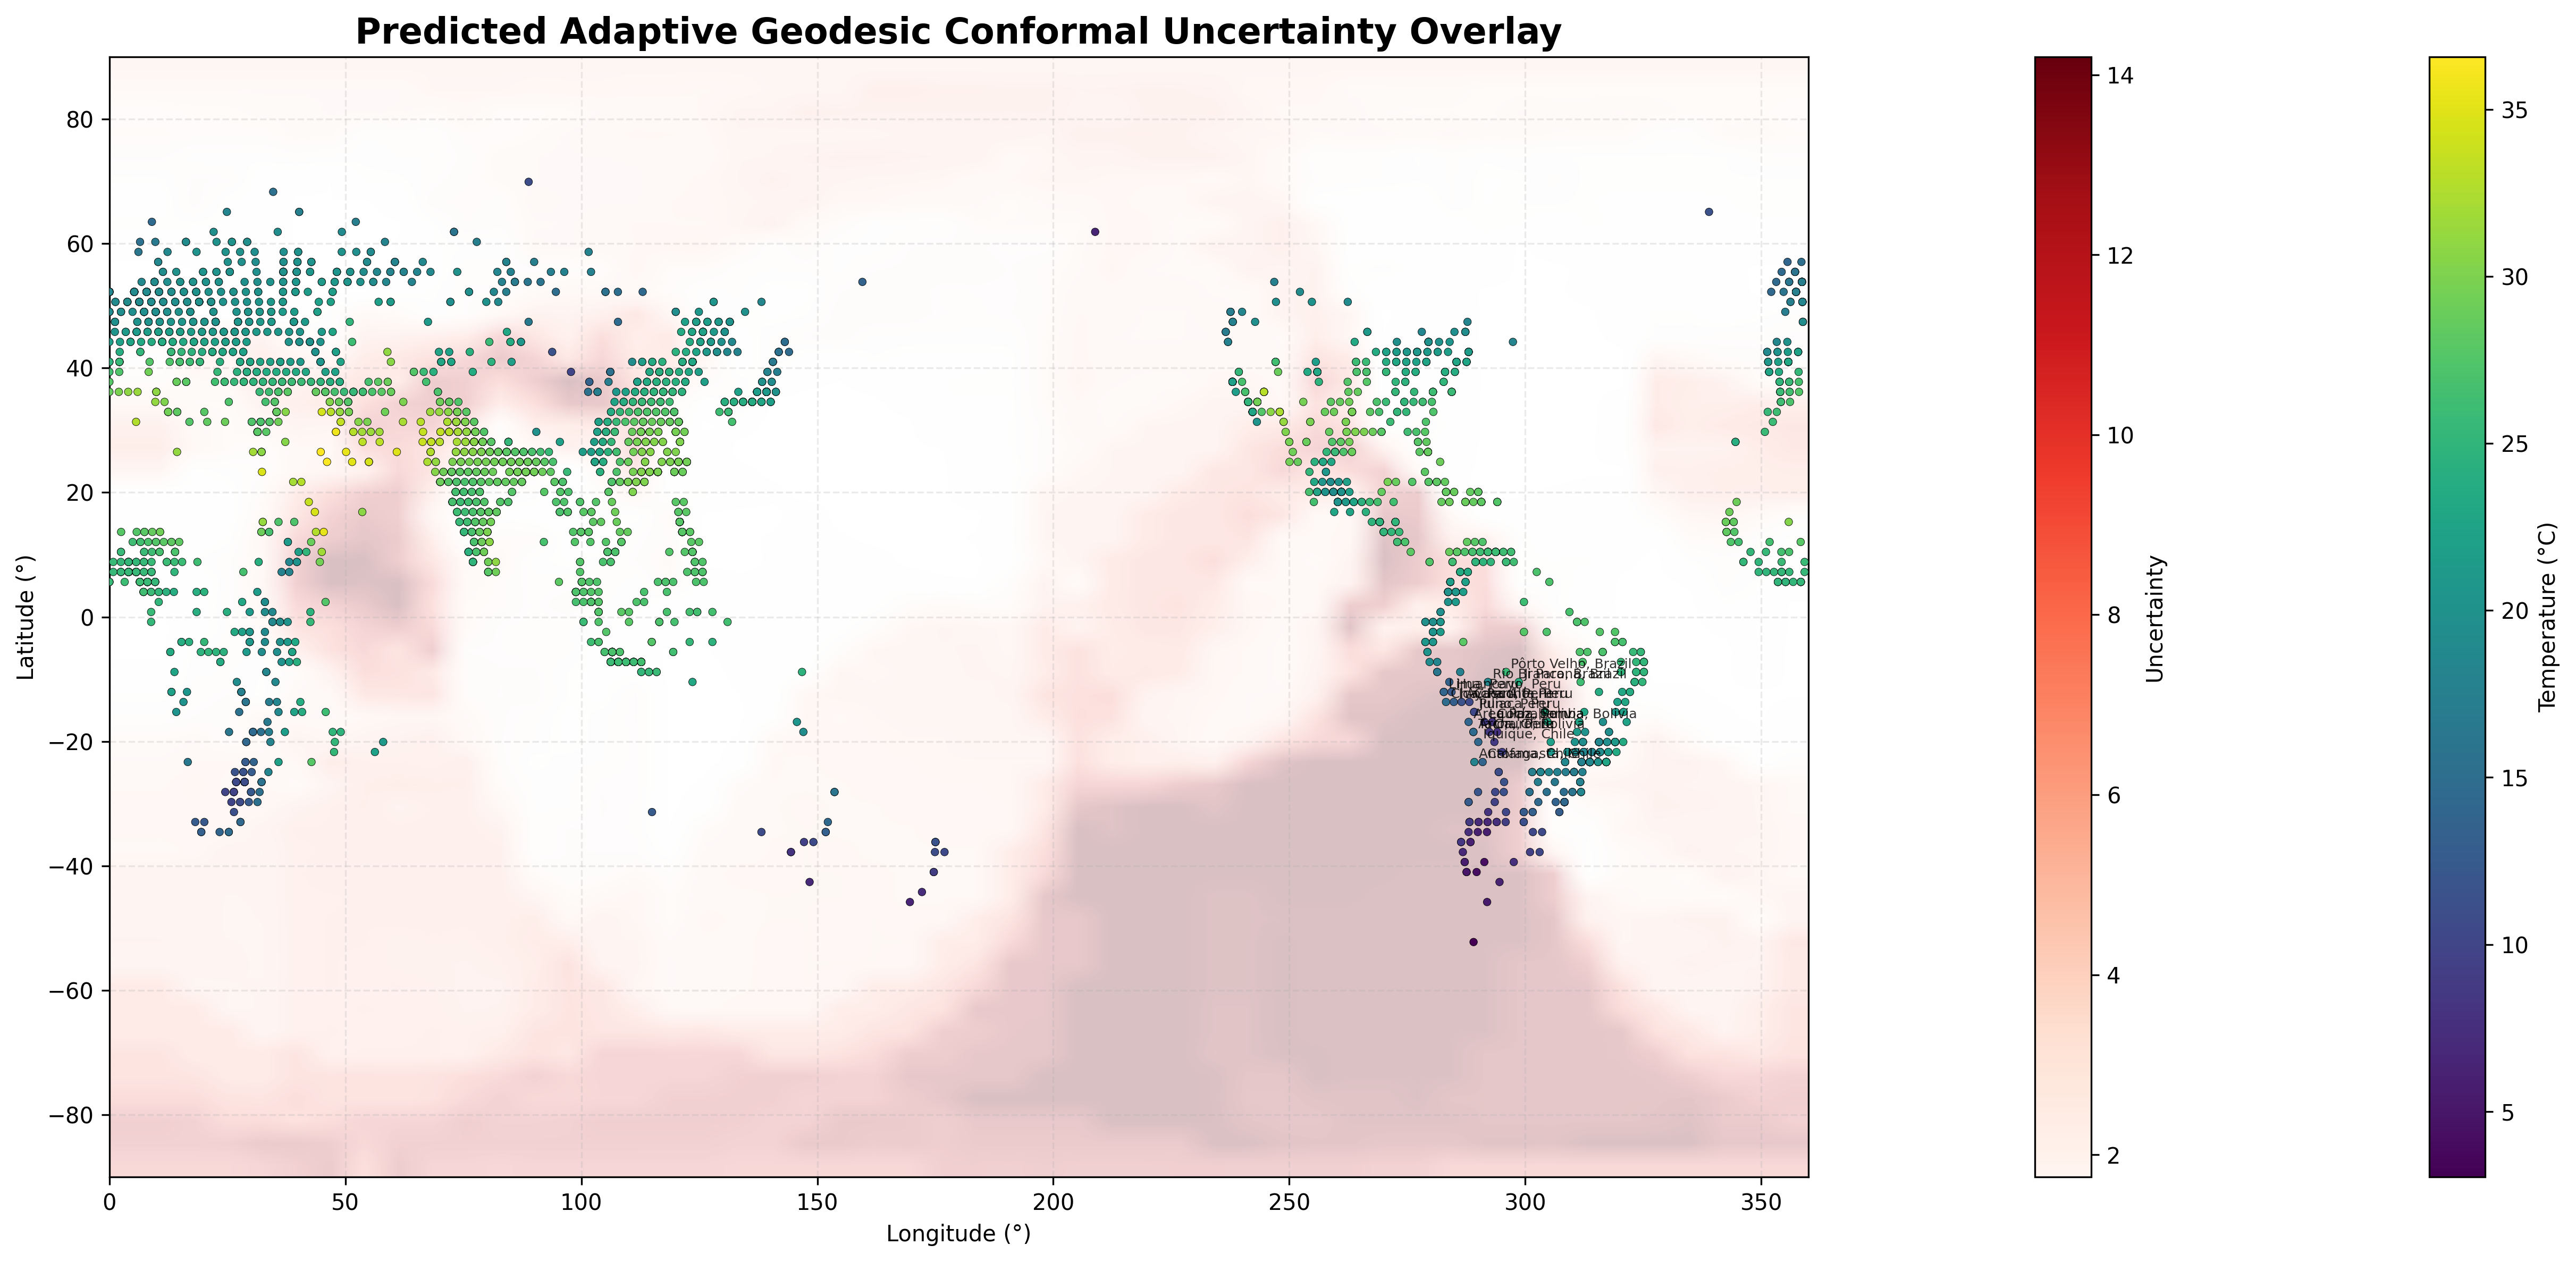
\includegraphics[width=\textwidth]{figures/opened_globe_uncertainty.png}
    \caption{Adaptive geodesic conformal uncertainty (red overlay) and predicted temperature (city markers) on an equirectangular (``opened-globe'') projection. Elevated uncertainty is visible in the sparsely-observed high-Andes region of South America, whose highest-uncertainty cities are labelled.}
    \label{fig:opened-globe}
\end{figure}
The main finding from the geographic analysis is related to \textbf{uncertainty}, rather than just the size of the reconstruction residuals. The cities were ranked based on their estimated difficulty $\hat\sigma(x)$, and the top $5\%$ were then examined (\cref{fig:opened-globe}). The full table is listed in \autoref{ch:appendix}. The twenty highest-uncertainty cities in the entire dataset are mostly concentrated in the high-altitude Andean region of Bolivia, Peru and northern Chile (\cref{fig:opened-globe}). Seventeen of the twenty highest-$\hat\sigma$ cities are from this region, including La Paz, Tacna, Arica, Puno, Juliaca, Arequipa, Cochabamba, Cusco, Ayacucho, Ica, Chincha Alta, Antofagasta, Iquique, Calama, Huancayo, Oruro and Chosica. The remaining three (Pôrto Velho, Rio Branco, Ji-Paraná) are located in the sparsely observed western Brazilian Amazon. Local observation density was also examined to understand the uncertainty results. This includes the number of other cities within $250$, $500$, and $1{,}000,\mathrm{km}$ and the great-circle distance to the $20$th-nearest city. The results show that the high-uncertainty Andean cities generally have only around 2-5 nearby cities within 250 km, while distances of approximately 800--1,400 km are needed to find 20 neighbouring cities. This indicates that these areas have much lower observation density compared with regions such as Europe, eastern China, and the eastern United States. The spatial sparsity provides evidence that limited local observations may contribute to higher estimated uncertainty. Fewer nearby observations mean less local information is available to support the reconstruction. For instance, the Andes also combine low observation density with a distinctive climate environment. High elevation can lead to strong temperature differences compared with lower-altitude locations at similar latitudes, which may be difficult for the smooth spherical harmonic model to capture accurately. The model's spatial resolution is mainly controlled by the global spherical harmonic degree $L$. It does not automatically increase the resolution specifically in areas with complex local terrain. Therefore, local geographic and climatic variation may remain difficult to model. The two possible explanations are consistent, with the observed high-uncertainty locations, insufficient local observation density and genuine physical structure that is not fully captured by the model. The adaptive conformal method also identifies these areas as having higher uncertainty, which suggests that the uncertainty estimates contain meaningful geographic information. However, these results do not prove that either mechanism directly causes the higher uncertainty.
% ============================================================

\chapter{Discussion}
\label{ch:discussion}

\section{Interpreting the coverage results}

The main empirical finding of this dissertation is that standard split conformal prediction over-covers easy regions and badly under-covers difficult regions, while the proposed adaptive method keeps coverage much closer to nominal 90\% across all difficulty levels (\cref{tab:tertile,tab:sixbin}). The same qualitative pattern was reported by \citet{amirishahbazi2026} for both of their case studies, despite the difference in problem structure discussed in \cref{sec:adaptation}. Therefore, the similarity suggests that the adaptive approach may work across different types of prediction problems. The key mechanism driving the improvement is the normalisation of nonconformity by a locally informative difficulty estimate, which can improve the allocation of interval width across different levels of difficulty. This is an empirical improvement rather than a formal theoretical guarantee of conditional coverage, since the formal conformal guarantee is for marginal coverage under the required exchangeability assumptions. The exact geometric construction is different, with previous work using geodesic caps for a manifold-valued response, while this dissertation is on scalar prediction intervals whose widths are determined using a geodesic-neighbourhood difficulty estimator. Despite this difference, the important component is whether the difficulty estimator is sufficiently informative. Therefore, the particular geometric implementation may be less important than obtaining a useful local estimate of prediction difficulty.
 
That said, the two settings are not equally challenging for the mechanism to succeed in. In this current dissertation setting, the covariate is the exact geographical location of each city. Coordinates are known directly and the geodesic $k$-NN neighbourhood used for $\hat\sigma(x)$ can therefore be computed directly on $S^2$. There is no additional uncertainty in determining the neighbourhood apart from numerical and geometric calculations. In \citeauthor{amirishahbazi2026}'s setting, both the covariate and response can involve noise or model-dependent uncertainty. The response is also manifold-valued, so $\hat\sigma(x)$ can be more complicated as errors from the base predictor may interact with the geometry of the manifold-valued response. 

The higher $r$ does not necessarily mean the proposed method is universally better. This gap between the correlation obtained here ($r = 0.634$) and \citeauthor{amirishahbazi2026}'s real-data case study ($r = 0.516$) has at least two plausible, non-exclusive explanations. The first is the setting difference just described: exact spatial coordinates, a scalar response, and direct geodesic neighbourhood calculation avoid the interaction between predictor error and output curvature present in \citeauthor{amirishahbazi2026}'s manifold-response setting. A second, non-exclusive explanation is that near-surface temperature is strongly spatially autocorrelated at the scale of tens to hundreds of kilometres, which may give a $k$-nearest-neighbour residual estimator a genuinely easier signal to exploit than for geomagnetic field anomalies, which may vary more locally. The present study cannot fully separate these two explanations, as doing so would require applying both methods to a common underlying field. The relative stability of $r$ across spherical harmonic degree ($r \approx 0.61$-$0.68$ for $L = 8$-$30$, \cref{tab:degree-robustness}) is weak but suggestive evidence that the correlation reflects the spatial structure of the temperature field rather than any single model configuration, though this is not conclusive. Therefore, the two correlation values should be compared as empirical results from different problem settings rather than as a direct ranking of the two methods.
 
\section{Why interval width is comparable, not just coverage}

The adaptive method's improvement is captured clearly in \cref{tab:main-coverage} where it improves coverage without producing wider intervals overall and its mean width is slightly narrower on average than the standard method ($4.59^\circ\mathrm{C}$ versus $4.65^\circ\mathrm{C}$). This is possible because the adaptive method redistributes width instead of just uniformly increasing it. It narrows intervals for easy-tertile locations while widening them for hard-tertile locations. Standard conformal uses a common interval width, even though prediction difficulty varies spatially. This means easy locations may receive intervals that are unnecessarily wide and difficult locations may receive intervals that are not wide enough. Adaptive conformal provides a more appropriate allocation of uncertainty. As a result, the overall mean interval width remains approximately the same, while producing a large improvement in the conditional-coverage metrics that the mean alone cannot capture. This is the same point that \citeauthor{amirishahbazi2026} make about their naive-coordinate baseline wasting prediction-region area rather than simply causing incorrect coverage. In the current scalar-response setting, a similar idea applies where uniform interval width does not account for different prediction difficulties. Therefore, the advantage of the adaptive method is not simply higher coverage. It provides more balanced conditional coverage, similar or slightly smaller average interval width, narrower intervals for easier locations, and wider intervals for genuinely difficult locations. This suggests that the adaptive method provides a more efficient allocation of uncertainty across the spatial domain.
 
\section{Computational considerations}

The pipeline's main computational costs in this dissertation come from three parts: (i) the five-fold cross-validated hyperparameter grid search over $21$ values of $\lambda$ and $5$ values of the Sobolev order $k$ at $L=26$, which requires $5\times21\times5=525$ fold-level model evaluations; (ii) the five-fold cross-validation used to construct the out-of-fold residual field for $\hat\sigma(x)$, which requires five additional model refits; and (iii) the degree-robustness experiment, which repeats these procedures at eight different values of $L$. For all repeated grid-search calculations, PyTorch is used for spherical-harmonic matrix operations, matrix multiplication, and regularised linear-system solving, while SciPy is used for associated Legendre-function evaluations performed on the CPU. Within each fold, the design matrix, Gram matrix $A^HA$, and right-hand side $A^H\hat f$ are computed once and reused across the different $(\lambda,k)$ combinations. This avoids repeatedly constructing the same matrices. The final model fit is performed separately using the NumPy/SciPy implementation. As the tested degree becomes larger, such as $L=30$, the size of the normal-equation system also increases, with dimension $(L+1)^2=961$. Compared with $729$ at $L=26$, this results in a larger linear system and higher computational cost. The experiments were feasible on the available computer hardware, although increasing the degree, substantially refining the hyperparameter grid, testing more Sobolev orders, or using more CV folds would increase the computational cost. However, once training and calibration are complete, evaluating the calibrated model at a new query point is comparatively inexpensive. This is because it only requires evaluation of the spherical-harmonic basis, estimation of the local difficulty from the precomputed residual field, and computation of the corresponding prediction interval. Overall, the training and model-selection process is more computationally expensive than prediction at a new point.
 
\section{Comparison with alternative spatial uncertainty quantification approaches}

It is worth investigating and comparing the conformal approach against the geostatistical alternative mentioned in \cref{ch:intro}, Gaussian Process/Kriging, a natural alternative from spatial statistics. A Gaussian Process produces a probabilistic prior over the spatial field, which requires a specifying covariance/kernel function (e.g. spherical Matérn). This kernel is used to represent assumptions about spatial correlation and smoothness. A Gaussian Process will therefore produce a full posterior predictive distribution, such as a predictive mean, variance and intervals directly. This is much richer than the conformal interval, but its uncertainty estimates depend heavily on the chosen kernel and noise model. So if the assumed covariance structure is wrong or misleading, the predictive variance may be poorly calibrated. This might potentially affect my data because of spatially varying/terrain-related temperature patterns documented in \cref{sec:geography}. The resulting posterior variance can be easily systematically miscalibrated with no finite-sample mechanism to correct it. In contrast, the conformal guarantee of \cref{sec:cp-background} holds regardless of model misspecification. In conclusion, a Gaussian Process provides richer probabilistic uncertainty, but its uncertainty is dependent on correctly specifying the spatial covariance structure. 

My approach takes a different route. It keeps the existing spherical harmonic reconstruction model and applies conformal prediction on top of that predictor. It does not require specifying a Gaussian Process covariance kernel. In my case, calibration residuals are used to determine the prediction interval. Therefore, the uncertainty calibration does not depend on the spherical harmonic model having a correctly specified probabilistic covariance structure. The conformal coverage guarantee is model-agnostic, but not assumption-free. The advantage is therefore reliable interval calibration without replacing or rebuilding the underlying spatial predictor. Conformal prediction sacrifices the full probabilistic output of a Gaussian Process, but provides a model-agnostic way to calibrate prediction intervals on the existing predictor.

Gaussian process regression is also computationally more demanding because its covariance matrix has dimension $n\times n$, with a cubic computational cost of $O(n^3)$ for a direct factorisation. In the present dataset, with $n=2{,}106$ training points, it is feasible to compute but the cost grows quickly with more observations. On the other hand, the spherical harmonic formulation works in a coefficient space with dimension $(L+1)^2$. Dense factorisation therefore has a worst-case complexity of $O(((L+1)^2)^3)=O((L+1)^6)$. This distinction is important because the two approaches scale with different quantities. The Gaussian Process approach is driven primarily by the number of observations, whereas the spherical harmonic calculation is driven primarily by the number of basis functions. For the present setting, where $L\ll n$, the latter provides a substantially smaller linear system. It should be noted that theoretical complexity does not necessarily equal actual runtime, because implementation, hardware, matrix structure, and approximation methods also matter. The conformal approach adopted in this dissertation therefore trades the fully probabilistic output of a Gaussian Process for a model-agnostic marginal coverage guarantee that can be applied to the existing spherical harmonic predictor without redesigning the underlying reconstruction model.

\section{Broader implications}

Going back to the practical motivation from the introduction \cref{ch:intro}, a downstream user is also expected to know where the reconstructed field can be trusted, as a single global accuracy measure is not enough. The tertile results in \cref{tab:tertile} show that standard conformal has a nominal coverage of 90\%, but the actual coverage in the highest-difficulty tertile is only 76.7\%. This is a substantial difference from the target coverage, with the under-coverage mainly concentrated in particular spatial regions across the dataset. The geographic analysis in \cref{sec:geography} suggests some possible physical and geographical reasons behind these patterns. A user may assume that a nominal 90\% interval provides roughly 90\% reliability everywhere, but the results show that coverage can vary across different levels of prediction difficulty. The greatest risk occurs in areas where the predictor is most uncertain. Therefore, the adaptive method improves the numerical results while also providing more informative uncertainty estimates for downstream users. For example, a regional climate analyst may need to decide whether the reconstructed field over the Bolivian Altiplano is reliable enough for further modelling. A decision-maker could also use this information to identify areas where additional monitoring could improve confidence in the reconstructed field. The spatial uncertainty map \cref{fig:opened-globe} helps to show how the model performs across different regions, providing information that is not captured by an overall accuracy metric.

Adaptive conformal prediction does not address every type of spatial uncertainty. The conformal guarantee applies to the data distribution represented by the calibration and test data. It relies on the relevant exchangeability assumption and does not extend to arbitrary unseen regions. For instance, open-ocean locations are outside the spatial regime represented by the training data, as the available observations are limited to land-based locations (\cref{ch:data}). Therefore, oceanic locations differ from the regions represented in the observed data. This makes the issue one of extrapolation and generalisation, rather than just calibration.

A narrow interval at an oceanic location may appear reassuring, but it does not necessarily mean that the prediction is accurate there. The conformal calibration does not validate performance in a regime that is absent from the calibration data. In \cref{fig:opened-globe}, the uncertainty appears visually unremarkable over some oceanic grid points. However, the current analysis does not establish why this occurs, so it should not be interpreted as evidence that the method underestimates oceanic uncertainty. It is important to distinguish between calibration and accuracy. Calibration refers to how reliable the prediction intervals are under the represented data distribution, while accuracy refers to how well the underlying prediction performs in a new or structurally different region. Therefore, a calibrated interval should not be interpreted as evidence that the model is accurate everywhere, especially in regions that are poorly represented or absent from the observations. As a result, users should interpret uncertainty maps together with the spatial coverage of the training and calibration data. Regions outside the observed data regime require additional validation or physical observations. The proposed method improves uncertainty calibration within the represented data distribution, but it does not eliminate the problem of extrapolation into regions that are not represented in the observations. This distinction is important when using the reconstruction and uncertainty maps in practice, as good conformal calibration does not mean that the model is accurate everywhere.

\section{Limitations}

Several additional limitations should be acknowledged. 

First, the underlying dataset itself is a spatial and temporal average (Berkeley Earth's monthly city-level average), rather than a direct physical measurement, so it is not appropriate to interpret the residuals as measurement error. The reconstruction and its uncertainty should be described as a model fit to this processed dataset, rather than to the underlying physical measurement itself. This issue was already mentioned for the point-estimate model earlier and is carried over without change by this uncertainty-quantification layer. 

Second, the difficulty estimator's cross-validated residual field is estimated using only $2{,}106$ training points, and its own accuracy does not remain perfectly stable as model complexity changes, as shown in \cref{fig:degree-robustness}. A larger or more geographically diverse dataset could potentially improve the estimation of $\hat\sigma(x)$ further. 

Third, the specific choice $k_\sigma=20$ for the difficulty-estimator neighbourhood size was taken directly from \citet{amirishahbazi2026}. No independent tuning process was conducted for this dataset; therefore, no sensitivity analysis over $k_\sigma$ was conducted.

Fourth, the adaptation described in \cref{sec:adaptation} illustrates the adaptation motivated by the structural mismatch between a scalar-response problem and a manifold-response framework. It should not be seen as a validated theoretical result similar to the theoretical result in \citeauthor{amirishahbazi2026}, which is already well established and proved for the manifold-response case. The coverage guarantee obtained here instead follows from the standard (Euclidean, locally-adaptive) split-conformal argument of \citet{lei2018} and \citet{romano2019}. The geodesic input-neighbourhood construction might be one possible choice of difficulty estimator when it is geometrically well motivated.

Fifth, the reported test-set metrics in \cref{sec:main-results,tab:sixbin} are computed from a single fixed calibration and test split. This is the same split used throughout \cref{ch:results}, rather than being averaged over repeated random splits as in \citeauthor{amirishahbazi2026}'s $300$-trial and $100$-trial Monte Carlo evaluations. For the current dataset, a single split is already enough to demonstrate the conditional miscalibration of the standard method and the improvement obtained with the adaptive method. This also matches how the base predictor itself was evaluated in the earlier dissertation. The coverage and interval-width results are based on one fixed calibration and test split. Both calibration and test sets contain $n_{cal}=n_{te}=351$. Therefore, the exact numerical values have some unavoidable sampling variability, and the reported 88\%, 90\%, width, etc. should not be interpreted as exact population-level quantities. The main qualitative pattern is repeated across all eight values of $L$, as shown in \cref{tab:degree-robustness}. Each degree involves separate model fitting, calibration, and evaluation. This provides some reassurance that the main finding is not specific to one particular model degree. However, the eight experiments do not use independent random data splits. They are based on the same underlying partition. Therefore, they should not be described as eight independent replications. They mainly demonstrate that the result is reasonably consistent when model complexity changes. This still supports the robustness of the qualitative pattern to the choice of $L$, but does not quantify how much the results would change under a different random train/calibration/test partition. Therefore, it provides weaker evidence than repeated random-split experiments. A stronger evaluation would repeat the complete experiment over multiple random splits. This would allow examination of variation in empirical coverage and mean interval width, and stability of the adaptive-vs-standard comparison. It could also report mean, standard deviation, and confidence intervals. This would provide uncertainty estimates for the performance metrics themselves. Compared with the prior work of \citeauthor{amirishahbazi2026}, which used repeated Monte Carlo trials, a similar repeated-trial evaluation would improve this experimental design. It would also provide stronger evidence for the generality of the numerical results. 
 
% ============================================================

\chapter{Conclusion and Future Work}
\label{ch:conclusion}

\section{Summary}

This dissertation extends the existing regularised spherical harmonic model by adding a spatially adaptive, distribution-free uncertainty quantification layer. 
The adaptive geodesic conformal prediction method from  \citet{amirishahbazi2026}  was originally designed for manifold-valued responses. However, in this dissertation, the method is adapted to scalar responses. The main adaptation idea is to change the original method where geometric information is moved from the output side to the input side. Then, the geodesic neighbourhoods on the sphere are used to estimate local prediction difficulty. The background chapter, \Cref{ch:background}, covers two main theoretical areas: Sobolev-regularised spherical harmonic regression and split conformal prediction, including its locally adaptive and geometry-aware extensions. The methodology chapter, \cref{ch:methodology}, explains how the adaptation works and why the adaptation is appropriate for a scalar climate field. \cref{tab:adaptation-summary} summarises the main changes required for the scalar-valued climate field. 

When compared against standard conformal prediction on real city-level temperature data, the adaptive method appears to deliver more uniform conditional coverage across the different levels of prediction difficulty. In the most challenging test-set tertile, standard conformal shows a 13.3 percentage-point shortfall in coverage. The adaptive method corrects this shortfall while still maintaining a comparable and slightly narrower mean interval width. The advantage remains stable across a wide range of spherical harmonic degrees ($L=8$ to $L=30$), with two different criteria for selecting $\lambda$. Geographic analysis shows that high uncertainty is concentrated mainly in the high Andes. Some higher uncertainty is also found in the western Amazon. The geographic pattern of the uncertainty also provides a reasonable physical explanation for the statistical results. One possible reason could be that the high Andes have sparse observation coverage and large elevation-related temperature variations. These local variations make it difficult for the smooth spherical harmonic model to capture the temperature field accurately. Therefore, the uncertainty estimates are supported by the coverage results. The areas flagged as higher-uncertainty also tend to line up with regions where accurate reconstruction was already expected to be harder. Taken together, these results suggest that spatially adaptive conformal prediction is statistically effective, practically interpretable, and genuinely useful as an uncertainty-quantification layer for spectral reconstruction of geophysical fields. Importantly, it can be added on top of the existing point-prediction pipeline without needing any major changes to it.
 
\section{Future work}

\paragraph{Vector fields.} The previous dissertation also developed a vector spherical harmonic model for divergence-free tangential vector fields that was used to model wind data. The response is truly a tangent vector on $S^2$ and this is exactly the context for which \citeauthor{amirishahbazi2026}'s adaptive geodesic conformal prediction was designed. Applying adaptive geodesic conformal prediction to this setting would not require the input/output adaptation made, while the geodesic distance between predicted and true wind directions could be used directly as the nonconformity score. The earlier dissertation found that the vector-field model needed a much higher spherical harmonic degree and denser observations than the scalar case. This suggests that a future study could combine the vector spherical harmonic model with adaptive geodesic conformal prediction. This would provide uncertainty information for wind vector-field reconstruction. 
 
\paragraph{Sensitivity to $k_\sigma$ and alternative difficulty estimators.} Future work should investigate whether the results really depend on the difficulty estimator chosen here. In this dissertation, $k_\sigma=20$ was adopted rather than systematically optimised. Several different $k_\sigma$ values could be tested to examine how changing $k_\sigma$ affects the coverage, interval width, conditional coverage, and estimated $\hat\sigma$. Besides, different ways of estimating local difficulty should be compared with possible alternatives such as using kernel-weighted geodesic neighbourhoods, giving closer observations more weight, using  a separate regression model to predict  $\hat\sigma$ or even other local spatial smoothing methods. The purpose is to determine whether the improvement comes specifically from the $k$-NN estimator or is a more general consequence of adaptive normalisation.

\paragraph{Temporal extension.} Both this dissertation and its predecessor treat the reconstruction problem as purely spatial, using a single monthly snapshot. Therefore, the current problem is essentially spatial. Real climate applications involve both spatial variation and temporal variation. Future work could extend the spherical harmonic predictor into a spatio-temporal model. One possible approach is to use spherical harmonic basis function for spatial structure and temporal basis functions for the temporal structure. The predecessor dissertation suggested the use of \textbf{Laguerre polynomials} as one possible temporal basis. Adding time introduces another issue that observations at nearby times are not necessarily exchangeable. Standard split conformal assumptions may therefore no longer be directly appropriate. Future work would need a conformal method designed for non-exchangeable or time-dependent data. One possible direction is the non-exchangeable conformal framework referenced by \citeauthor{amirishahbazi2026}. This could move the framework from reconstructing one spatial snapshot toward uncertainty-aware climate forecasting. In conclusion, adding time would make the framework more relevant to real forecasting, but would also require dealing with temporal dependence and non-exchangeability.

\paragraph{Anisotropic regions.} Both this dissertation's intervals and \citeauthor{amirishahbazi2026}'s geodesic caps are isotropic, meaning they do not allow the uncertainty to be larger in one direction, for example, along a mountain range than another. Constructing anisotropic, still-valid conformal regions is noted as an open problem by \citeauthor{amirishahbazi2026} and remains open here as well. Given the pronounced elevation-aligned structure observed in \cref{sec:geography}, anisotropic uncertainty regions could potentially provide more spatially realistic uncertainty regions, better use of available prediction-region area, and more interpretable uncertainty around geographically structured features. Instead of only changing the size of uncertainty according to local difficulty, future methods could also change its shape according to local geographical direction.

% ============================================================


%%%%%%%%%%%%%%%%%%%%%%%%%%%%%%%%%%%%%%%%%%%%%%%%%%%%%%%%%%%%%%%%%%%%%%%%%%%%%%%%%%%%
\bibliography{references} % references.bib

%%%%%%%%%%%%%%%%%%%%%%%%%%%%%%%%%%%%%%%%%%%%%%%%%%%%%%%%%%%%%%%%%%%%%%%%%%%%%%%%%%%%
\begin{appendices}
\chapter{Additional Results}
\label{ch:appendix}

\section{Highest-uncertainty cities}

\Cref{tab:appendix-cities} lists the twenty test-region cities with the highest estimated difficulty $\hat\sigma(x)$, with the local observation-density diagnostics mentioned in \cref{sec:geography}, present the number of other cities within $250\,\mathrm{km}$, $500\,\mathrm{km}$ and $1{,}000\,\mathrm{km}$, and the great-circle distance required to reach the $20$th-nearest city.
\begin{table}[H]
\centering
\caption{Twenty highest-uncertainty cities, with local observation-density diagnostics.}
\label{tab:appendix-cities}
\scriptsize
\begin{tabular}{lccccc}
\toprule
City (Country) & $\hat\sigma$ & Within 250 km & Within 500 km & Within 1000 km & Dist.\ to 20th NN (km) \\
\midrule
La Paz (Bolivia) & 5.30 & 2 & 11 & 21 & 948.7 \\
Tacna (Peru) & 5.27 & 2 & 7 & 22 & 952.4 \\
Arica (Chile) & 5.27 & 2 & 7 & 22 & 952.4 \\
Puno (Peru) & 5.25 & 2 & 9 & 22 & 894.0 \\
Juliaca (Peru) & 5.25 & 2 & 9 & 22 & 894.0 \\
Arequipa (Peru) & 5.25 & 4 & 10 & 23 & 839.4 \\
Cochabamba (Bolivia) & 5.25 & 3 & 9 & 21 & 945.1 \\
Cusco (Peru) & 4.95 & 4 & 8 & 23 & 828.1 \\
P\^orto Velho (Brazil) & 4.90 & 0 & 2 & 4 & 1307.6 \\
Rio Branco (Brazil) & 4.85 & 1 & 2 & 19 & 1029.3 \\
Ayacucho (Peru) & 4.66 & 3 & 11 & 23 & 808.0 \\
Ica (Peru) & 4.52 & 4 & 11 & 23 & 903.2 \\
Chincha Alta (Peru) & 4.40 & 5 & 7 & 21 & 991.2 \\
Antofagasta (Chile) & 4.35 & 1 & 2 & 23 & 834.0 \\
Ji Paran\'a (Brazil) & 4.28 & 1 & 2 & 8 & 1366.2 \\
Iquique (Chile) & 4.25 & 2 & 10 & 21 & 907.0 \\
Calama (Chile) & 4.20 & 1 & 6 & 23 & 780.3 \\
Huancayo (Peru) & 4.17 & 5 & 10 & 24 & 907.3 \\
Oruro (Bolivia) & 4.16 & 4 & 11 & 20 & 966.5 \\
Chosica (Peru) & 3.84 & 3 & 7 & 22 & 981.3 \\
\bottomrule
\end{tabular}
\end{table}

\section{Software}

All modelling, calibration and figure generation was implemented in Python by using \texttt{NumPy} and \texttt{SciPy} for the core spherical-harmonic and associated-Legendre computations, whereas \texttt{PyTorch} used for GPU-accelerated design-matrix assembly and linear solves during hyperparameter search and grid reconstruction. In addition, \texttt{pandas} and \texttt{scikit-learn} were used for data handling and cross-validation splitting, while \texttt{Matplotlib}/\texttt{seaborn} was used for visualisation.

All coding used to produce the results and figures in this dissertation was carried out in Python. The full code is available at the following GitHub repository: \url{https://github.com/szeying-code/temperature-scalar-field-reconstruction-with-uncertainty-}. 

\section{Reproducibility details}

For reproducing details, the following settings specify the main fixed parameters used in the pipeline reported in \cref{ch:results}. A random seed of $42$ is used for all data-splitting operations, at the four-way train/validation/calibration/test split of \cref{ch:data}. The five-fold cross-validation folds used both for hyperparameter search and for the difficulty-estimator residual field, with target coverage level of $\alpha=0.1$ throughout, and a difficulty-estimator neighbourhood size of $k_\sigma=20$. A numerical floor of $\epsilon=10^{-6}$ on $\hat\sigma(x)$ applied to avoid division by zero in the normalised nonconformity score. The finite-sample-corrected conformal quantile level $\lceil(1-\alpha)(n_{cal}+1)\rceil/n_{cal}$ with the conservative (\texttt{"higher"}) interpolation rule implemented for empirical quantile estimation.

The calibration threshold obtained with $L=26$ model in \cref{sec:main-results} was $\hat q_\alpha = 2.389$, and the adaptive interval half-width at any query point was then $\hat q_\alpha\hat\sigma(x)$. This threshold of $\hat q_\alpha = 2.389$ is then used with the local difficulty estimate $\hat\sigma(x)$ to determine the interval width. This fixed model prediction intervals can be reconstructed using the calibration threshold $\hat q_\alpha = 2.389$, with the fitted coefficient vector $v$ and the stored training-set out-of-fold residual field used to calculate $\hat\sigma(x)$. Thus, it will be unnecessary to repeat the calibration procedure to make the specific numerical results in \cref{ch:results} reproducible. The accompanying code are able to use the same fixed values to reproduce the reported prediction intervals and results. This prevent changes caused by stochastic variation in cross-validation fold assignment or grid-search order.


\end{appendices}

\end{document}
